% --- Supplement starts ---
\clearpage
\onecolumngrid % optional

% --- SI title block (kept on the page, not in the SI ToC) ---
\begin{center}
  \textbf{\large Supplementary Information for}\\[1ex]
  \textbf{\large ``Programmable Quantum Matter: Heralding Large Cluster States in Driven Inhomogeneous Spin Ensembles''}
\end{center}

% (Optional) put one SI line in the MAIN ToC:
\addcontentsline{toc}{section}{Supplementary Information}

% --- Start SI-only ToC after the SI header entry to avoid duplicates ---
\addtocontents{toc}{\protect\SIonlyTOCstart}

\begingroup
\makeatletter
  % Switch flips to "print" once the marker above is encountered in .toc
  \newif\ifSIonly@print
  \SIonly@printfalse
  \def\SIonlyTOCstart{\SIonly@printtrue}

  % Gate the ToC entries so we ignore everything before the marker
  \let\SIold@section\l@section
  \def\l@section#1#2{\ifSIonly@print \SIold@section{#1}{#2}\fi}

  \@ifundefined{l@subsection}{}{%
    \let\SIold@subsection\l@subsection
    \def\l@subsection#1#2{\ifSIonly@print \SIold@subsection{#1}{#2}\fi}
  }
  \@ifundefined{l@subsubsection}{}{%
    \let\SIold@subsubsection\l@subsubsection
    \def\l@subsubsection#1#2{\ifSIonly@print \SIold@subsubsection{#1}{#2}\fi}
  }

  % Rename the default "CONTENTS" heading rather than adding your own section:
  \def\contentsname{Contents (Supplementary Information)}

  \tableofcontents
\makeatother
\endgroup




% Reset counters
\setcounter{section}{0}
\setcounter{equation}{0}
\setcounter{figure}{0}
\setcounter{table}{0}

% Use "S" prefix for clarity
\renewcommand{\thesection}{S\arabic{section}}
\renewcommand{\thefigure}{S\arabic{figure}}
\renewcommand{\thetable}{S\arabic{table}}
%\renewcommand{\theequation}{S\arabic{equation}}

% ALSO fix hyperlink anchors
\renewcommand{\theHsection}{S\arabic{section}}
\renewcommand{\theHfigure}{S\arabic{figure}}
\renewcommand{\theHtable}{S\arabic{table}}
%\renewcommand{\theHequation}{S\arabic{equation}}



\clearpage


\section{Strain Driving of Group-IV Color Centers in Diamond}

% --- Supplement ends ---



% \subsection{General Hamiltonian}

% \textbf{Here, we'd need to put a general form of the full matrix Hamiltonian for group IV, to be consistent with System Description in the main text. It would mean an Hamiltonian similar to the SiV one, but including neglected terms (Ag1, Egy...), }

\subsection{Monotonic Strain Window for the \(\mathrm{SiV}^{-}\) Center}

As stated in the main text, Algorithm 1 requires a control parameter that drives every optical qubit monotonically and injectively past a global laser frequency $f_L$. This section details the simulation that confirms
such an operational window exists for an ensemble of negatively charged silicon-vacancy (\(\mathrm{SiV}^{-}\)) centers, a
state-of-the-art solid-state platform. The simulation models the spin-conserving $C_2$ optical transition of an
inhomogeneous \(\mathrm{SiV}^{-}\) ensemble under an applied quasi-static strain.

\subsubsection{Simplified Model for the \(\mathrm{SiV}^{-}\) Center}
% The simulation applies the general Hamiltonian from Sec.~I.A to the specific case of the \(\mathrm{SiV}^{-}\). 

% Here, the matrix representation of $\hat{\mathcal{H}}_i^{\text{GS/ES}}$ is written in the basis of SO eigenstates $\{ \ket{e_{g/u-} \downarrow} , \ket{e_{g/u+} \uparrow} , \ket{e_{g/u+} \downarrow} , \ket{e_{g/u-} \uparrow} \}$ with the even (`gerade') parity orbitals ($g$) corresponding to the GS manifold and the odd (`ungerade') parity orbitals ($u$) to the ES manifold. The strain interaction is assumed to be dominated by $\epsilon_{E_{gx},i}^{dc} = d ( \epsilon_{xx} - \epsilon_{yy} ) + f \epsilon_{zx} $, with $d$ and $f$ the relevant strain-susceptibilities. The SO interaction is characterized by the SO coupling strength $\lambda_{\text{SO}}^{\text{GS/ES}}$. The Zeeman interaction describes the coupling of the orbital and spin angular momenta to a uniform magnetic field $\Vec{B}=B_x \Vec{1}_x + B_z \Vec{1}_z$ through their respective gyromagnetic ratios $\gamma_L$ and $\gamma_S$.



We adopt a set of simplifying assumptions consistent with experimental work performed by Meesala, \textit{et al.} \cite{PhysRevB.97.205444}: the model considers only transverse-oriented emitters where the strain tensor is assumed to be dominated by the $\epsilon_{yy}$ component. The energy level diagram for the \(\mathrm{SiV}^{-}\), showing the ground state (GS), excited state (ES), and the relevant optical transitions (\(\mathrm{C}_1\)-\(\mathrm{C}_4\)), is shown in Figure~\ref{fig:siv_levels}.


% where the strain tensor is dominated by the $\epsilon_{yy}$ component. The energy level diagram for the \(\mathrm{SiV}^{-}\), showing the ground state (GS), excited state (ES), and the relevant optical transitions (\(\mathrm{C}_1\)-\(\mathrm{C}_4\)), is shown in Figure~\ref{fig:siv_levels}.

\begin{figure}[h!]
    \centering
    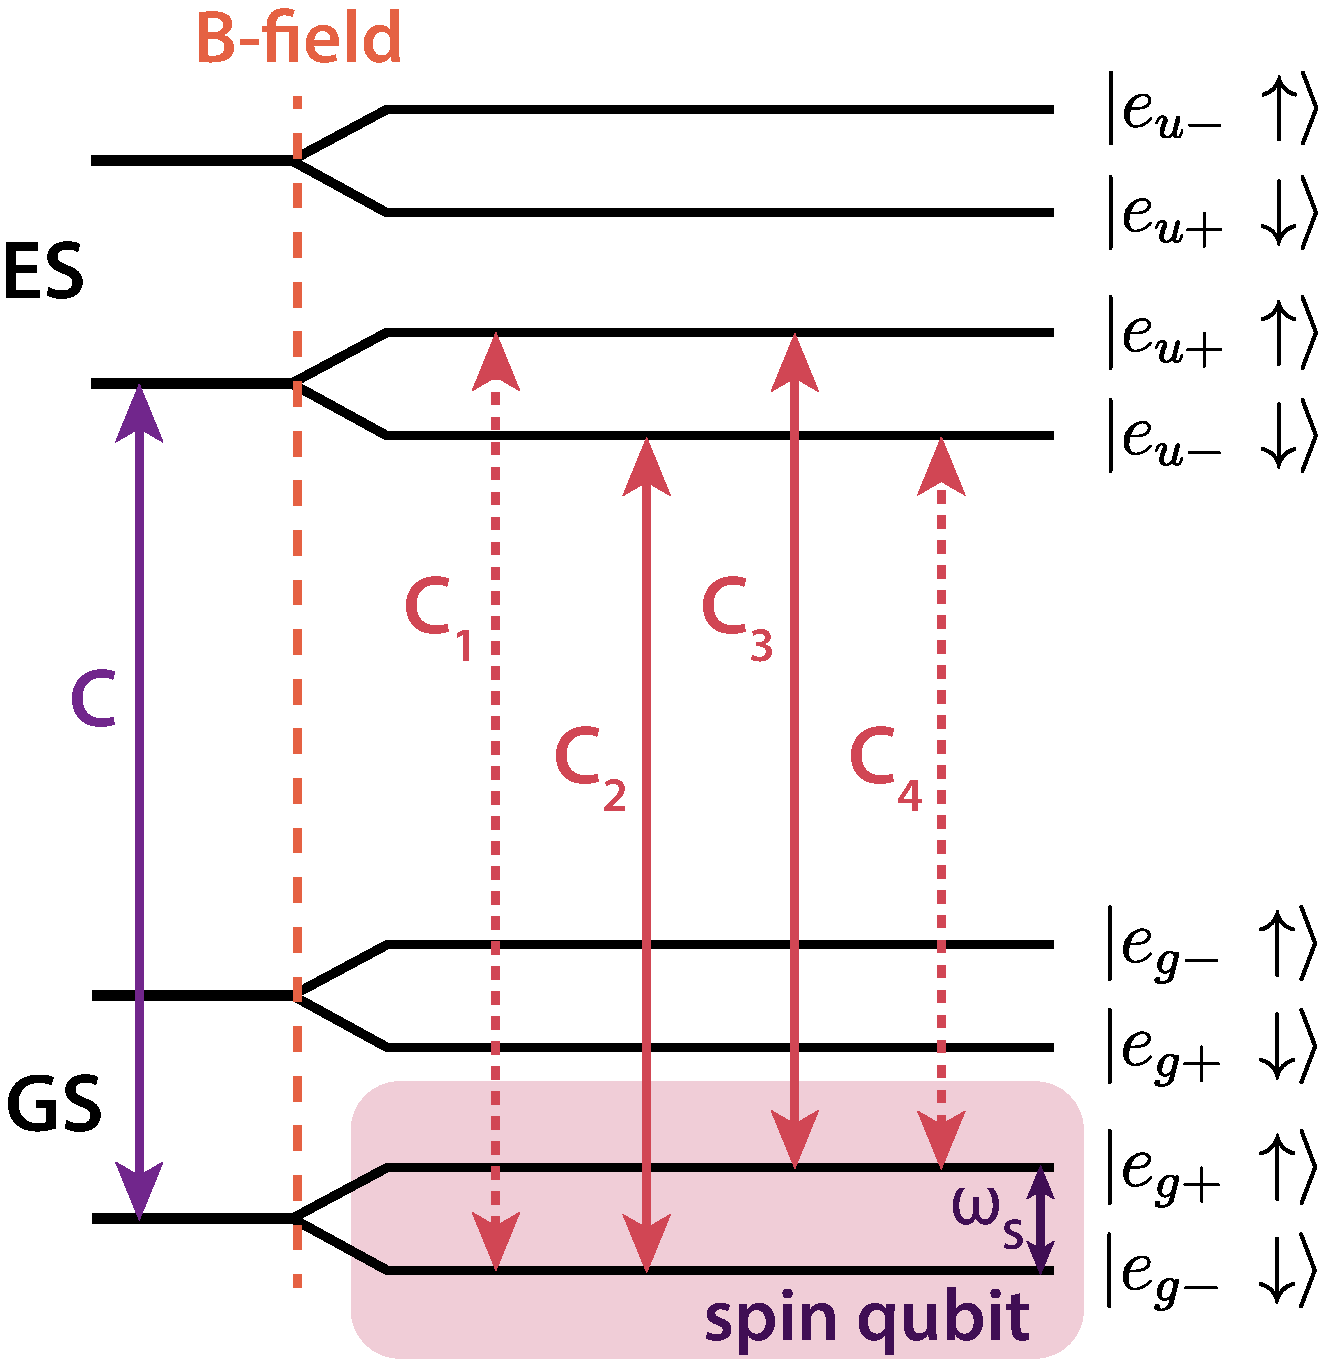
\includegraphics[width=0.5\textwidth]{figs/SI_Fig_1.pdf}
    \caption{\textbf{Energy level diagram for the \(\mathrm{SiV}^{-}\) center.} The diagram illustrates the fundamental energy level structure of the \(\mathrm{SiV}^{-}\) center. The ground (GS) and excited (ES) state manifolds are split by the spin-orbit interaction. An external magnetic field further splits each orbital branch into spin-up ($\uparrow$) and spin-down ($\downarrow$) sublevels via the Zeeman effect. The two lowest-energy ground state sublevels form the spin qubit, with transition frequency $\omega_s$. The simulation specifically calculates the frequency of the spin-conserving $C_2$ optical transition.}
    \label{fig:siv_levels}
\end{figure}

Under the additional assumption of the specific strain environment, the Hamiltonian governing these levels simplifies significantly. The SO interaction is characterized by the SO coupling strength $\lambda_{\text{SO}}^{\text{GS/ES}}$. The Zeeman interaction describes the coupling of the orbital and spin angular momenta to a uniform magnetic field $\Vec{B}=B_x \Vec{1}_x + B_z \Vec{1}_z$ through their respective gyromagnetic ratios $\gamma_L$ and $\gamma_S$. Finally, this yields the following Hamiltonian, written in the basis of spin-orbit eigenstates $\{ |e_{-} \downarrow\rangle , |e_{+} \uparrow\rangle , |e_{+} \downarrow\rangle , |e_{-} \uparrow\rangle \}$ for a given manifold (GS/ES) and center $i$:
\begin{align}
 & \hat{\mathcal{H}}_i^{\text{GS/ES}} \nonumber \\
 & =
 \begin{pmatrix}
    - \frac{\lambda_{\text{SO}}}{2} - \gamma_L B_z - \gamma_S B_z & 0 & \epsilon_{E_{gx}} & \gamma_S B_x \\
    0 & - \frac{\lambda_{\text{SO}}}{2} + \gamma_L B_z + \gamma_S B_z & \gamma_S B_x & \epsilon_{E_{gx}} \\
    \epsilon_{E_{gx}} & \gamma_S B_x & \frac{\lambda_{\text{SO}}}{2} + \gamma_L B_z - \gamma_S B_z & 0 \\
    \gamma_S B_x & \epsilon_{E_{gx}} & 0 & \frac{\lambda_{\text{SO}}}{2} - \gamma_L B_z + \gamma_S B_z 
 \end{pmatrix}
\end{align}
Here, the primary effect of strain is captured by the off-diagonal $\epsilon_{E_{gx}}$ term, approximated by $\epsilon_{E_{gx}}=- d_{gs/es}\, \epsilon_{yy}$.

\subsubsection{Simulation and Parameters}
To accurately model the inhomogeneous ensemble, we must define a statistical distribution of the static fabrication biases, $\epsilon_{E_{gx},i}^{\text{bias}}$. We derive the the standard deviation, $\sigma_\epsilon$, of this distribution from experimentally measured inhomogeneous broadening of the \(\mathrm{SiV}^{-}\) C-transition, which is reported by Meesala, \textit{et~al.}~\cite{PhysRevB.97.205444} to have a standard deviation of $\sigma_f \approx 31$~GHz for centers in nanofabricated devices. In the low-strain limit, the optical frequency shift is approximately linear with strain:
\begin{equation}
    \Delta f \approx (d_{es} - d_{gs}) \epsilon_{E_{gx}} \equiv \Delta d \cdot \epsilon_{E_{gx}}
\end{equation}

Using the susceptibility parameters from Table~\ref{tab:simparams}, the differential susceptibility is $\Delta d = (1.8 - 1.3) \times 10^{15}$~Hz/strain = 0.5~PHz/strain. This allows us to estimate the standard deviation of the underlying strain distribution:
\begin{equation}
    \sigma_{\epsilon} = \frac{\sigma_f}{\Delta d} = \frac{31 \times 10^9 \text{ Hz}}{0.5 \times 10^{15} \text{ Hz/strain}} \approx 6 \times 10^{-5}
\end{equation}
Based on this calculation, we adopt a rounded value of $\sigma_\epsilon = 6 \times 10^{-5}$ for the simulation. The static biases $\epsilon_{E_{gx},i}^{\text{bias}}$ are therefore drawn from the Gaussian distribution $\mathcal{N}(0, \sigma_\epsilon)$. The frequency of the \(\mathrm{C}_2\) transition is then computed for each center by numerically diagonalizing the simplified Hamiltonian for the total strain $\epsilon_{E_{gx},i} = \epsilon_{E_{gx},i}^{\text{bias}} + \epsilon_{E_{gx}}^{\text{dc}}$ and parameter values from Table \ref{tab:simparams}. The results, plotted as the detuning $\Delta f$ in Figure 10 of the main text, confirm that a common monotonic window exists for the simulated inhomogeneous ensemble.

\begingroup
 \renewcommand{\thetable}{S\arabic{table}}
 \setcounter{table}{0}
 \begin{table}[h!]
    \centering
    \vspace{4pt}
    \begin{tabular}{|l|c|l|}
      \hline
      \textbf{Quantity} & \textbf{Symbol} & \textbf{Value} \\ \hline
      spin–orbit split (ground)   & \(\lambda^{\text{gs}}_{\text{SO}}\) & \(46~\mathrm{GHz}\) \\
      spin–orbit split (excited)  & \(\lambda^{\text{es}}_{\text{SO}}\) & \(255~\mathrm{GHz}\) \\
      orbital \(g\)--factor       & \(g_L\)                         & \(1.4\) \\
      spin \(g\)--factor          & \(g_S\)                         & \(14\) \\
      magnetic field              & \(B\)                           & \(0.17~\mathrm{T}\) (in the \(xz\) bisector) \\
      strain coefficient (GS)     & \(d_{gs}\)                      & \(1.3\times10^{15}~\mathrm{Hz/strain}\) \\
      strain coefficient (ES)     & \(d_{es}\)                      & \(1.8\times10^{15}~\mathrm{Hz/strain}\) \\
      bias strain distribution, std. dev. & \(\sigma_\epsilon\)             & \(6\times10^{-5}\) \\
      assumed strain components   & ---                             & \(\epsilon_{yy}\neq0,\; \epsilon_{xx}=\epsilon_{xz}=0\) \\
      \hline
    \end{tabular}
    \caption{Parameters used in the \(\mathrm{SiV}^{-}\)-specific simulation. Adapted from \cite{PhysRevB.97.205444}.}
    \label{tab:simparams}
 \end{table}
\endgroup

\subsection{Strain Driving Simulations}
\label{sec:straindriving}

Strain driving \(\hat{\mathcal{H}}^{\text{drive}}(\varphi=\pi-\phi)\) can be used to implement arbitrary single-qubit gates $\hat{\mathcal{U}}^{\text{ideal}}(\theta,\phi)$ on the spin qubit defined by the \(\mathrm{SiV}^{-}\) $\hat{\mathcal{H}}^{\text{GS}}$ lowest two eigenstates. The parameter $\theta$ is determined by the Rabi drive strength $\Omega$ and the evolution time. The parameter $\phi$ is controlled using the phase $\varphi$ of the strain drive. Fig~\ref{fig:strain_driving} illustrates three cases of those arbitrary gates: rotation on the Bloch sphere around the x-axis (\ref{fig:strain_driving}.i), y-axis (\ref{fig:strain_driving}.ii) and xy-bisector (\ref{fig:strain_driving}.iii). Here, the static strain $\epsilon_{Egx}^{\text{dc}}$ is set to $4\times10^{-6}$ and the applied magnetic field $\vec{B}$ to $0.25\text{T}\times\frac{1}{\sqrt{2}}(\vec{1}_x+\vec{1}_z)$. In all three cases, fidelities above 99.7\% are achieved for various initial states  (FIG. \ref{fig:strain_driving} (c)). FIG. \ref{fig:strain_driving} (a) shows that Rabi oscillations are induced by strain driving after initializing the qubit in its ground state. The strain drive amplitude $\epsilon_{Egx}^{\text{ac}}$ is picked as $1.560\times10^{-6}$, $1.560\times10^{-6}$ and $1.553\times10^{-6}$ respectively, in order to realize $\Omega=200$ Mrad/s. The slight population of the two upper levels contributes to the imperfect fidelity of the Rabi oscillations between the two lowest energy levels. 

\begin{figure}[h!]
    \centering
    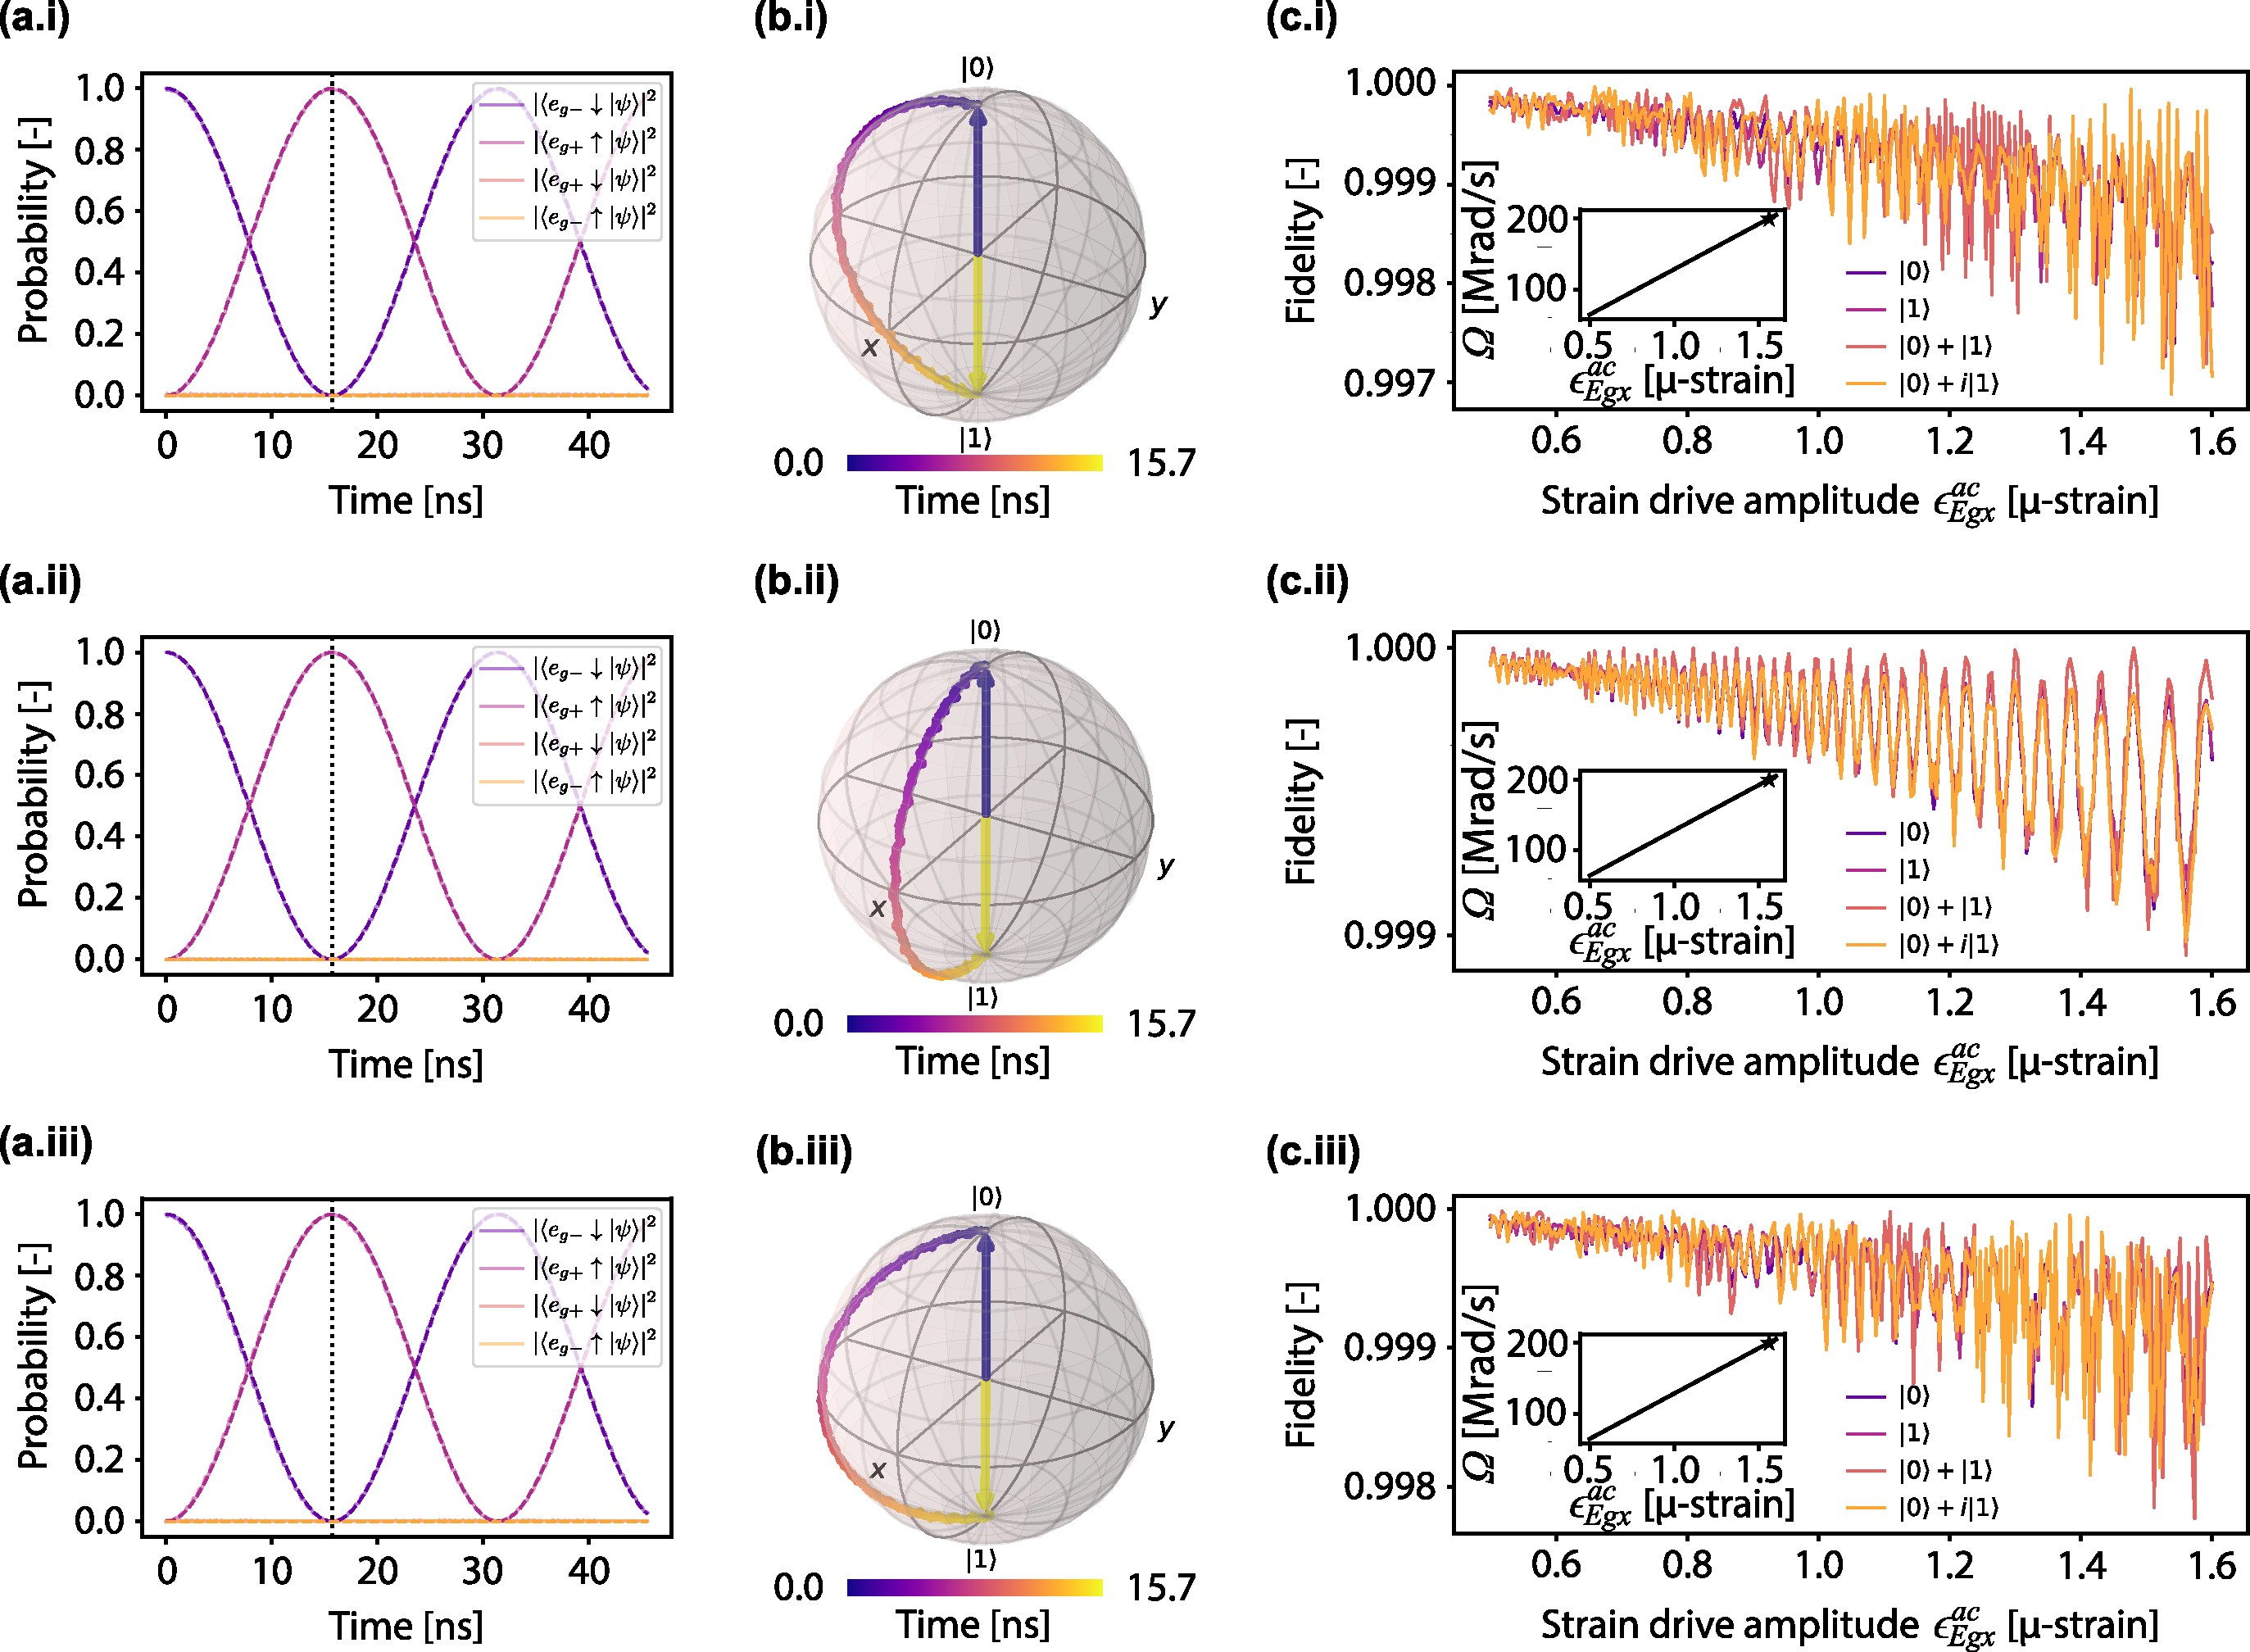
\includegraphics[width=\textwidth]{figs/SI_Fig_2.pdf}
    \caption{\textbf{Arbitrary single-qubit gates $\mathbf{\hat{\mathcal{U}}(\theta,\phi)}$ implemented by strain driving.} \textbf{(a)} System evolution under strain drive Hamiltonian $\hat{\mathcal{H}}^{\text{drive}}$ for initial state $|0\rangle = |e_{g-}\downarrow\rangle$. Rabi oscillations between the eigenstates of the bottom two energy levels can be observed. The colored dashed lines correspond to the best ideal Rabi oscillations fit. The strain drive amplitude $\epsilon_{Egx}^{ac}$ is chosen to realize a Rabi drive strength $\Omega$ of 200 Mrad/s. The black vertical dotted line indicates the time at which a $\pi$ rotation is achieved. \textbf{(b)} Bloch sphere representation of the time evolution during this $\pi$ rotation gate. The arrows mark the initial and final state. \textbf{(c)} State fidelity between the state after evolution under the strain drive Hamiltonian and the ideal final state, for different initial states. \textbf{(inset of (c))} Optimal fit of the Rabi drive strength for a set strain drive amplitude. The star indicates the point that realizes $\Omega$ of 200 Mrad/s. Note that arbitrary single-qubit gates can be implemented. Here the results are shown for \textbf{(i)} rotations around the x-axis ($\hat{\mathcal{U}}(\theta,\phi=0)$) implemented by $\hat{\mathcal{H}}^{\text{drive}}(\varphi=\pi)$, \textbf{(ii)} rotations around the y-axis ($\hat{\mathcal{U}}(\theta,\phi=\pi/2)$) implemented by $\hat{\mathcal{H}}^{\text{drive}}(\varphi=\pi/2)$ and \textbf{(iii)} rotations around the xy-bisector ($\hat{\mathcal{U}}(\theta,\phi=\pi/4)$) implemented by $\hat{\mathcal{H}}^{\text{drive}}(\varphi=3\pi/4)$.},
    \label{fig:strain_driving}
\end{figure}

\section{Concatenated Composite Pulses}

\subsection{Concept}

Composite-pulse control replaces an elementary single-qubit gate
\(\hat{\mathcal{U}}_{\mathrm{ideal}}(\theta,\phi)\), defined as
\[
\hat{\mathcal{U}}_{\mathrm{ideal}}(\theta,\phi)= \exp\!\left[-\tfrac{i}{2}\theta\left(\cos\phi\,\hat\sigma_x + \sin\phi\,\hat\sigma_y\right)\right],
\]
with a short sequence of rotations
\(R(\theta_i,\phi_i)\)
whose combined propagator suppresses systematic errors to first order.
In a concatenated composite pulse (CCCP) \cite{Bando2012Concatenated} an \emph{outer} composite
sequence that cancels one error (here the amplitude / pulse-length error, PLE) is
nested with an \emph{inner} sequence that cancels the complementary
off-resonance error (ORE) while preserving the residual effect of PLE to
first order, the residual-error-preserving (REP) property.
Because the inner block then behaves like an effective single rotation
for PLE, the concatenation is first-order robust to both PLE and ORE.
The construction is summarised schematically in Fig.~\ref{fig:schematic_rCinBB}.

\subsection{Reduced CORPSE-in-BB1 (rCinBB) Sequence}

The four-pulse BB1 outer sequence \cite{WIMPERIS1994221} is written
\[
\hat{\mathcal{U}}_{\mathrm{BB1}}(\theta,\phi)=
\prod_{i=1}^{4} R(\theta_i,\phi_i),
\]
where \((\theta_1,\phi_1)\)–\((\theta_3,\phi_3)\) are given in
Table~\ref{tab:S2_theta_phi_CCCP} and \((\theta_4,\phi_4)=(\theta,\phi)\).
The three-pulse CORPSE inner block \cite{PhysRevA.67.042308},
\(\hat{\mathcal{U}}_{\mathrm{CORPSE}}(\theta,\phi)
 =R(\theta_4,\phi_4)R(\theta_5,\phi_5)R(\theta_6,\phi_6)\),
cancels ORE and is REP-PLE.
Because the first three BB1 rotations already form a trivial
\(\pi\text{–}2\pi\text{–}\pi\) block that is REP-ORE, only the
\emph{fourth} BB1 rotation must be replaced by CORPSE.
The resulting six-pulse reduced CinBB operator is therefore
\[
\hat{\mathcal{U}}_{\text{rCinBB}}(\theta,\phi)=
\prod_{i=1}^{6} R(\theta_i,\phi_i),
\]
with parameters collected in Table~\ref{tab:S2_theta_phi_CCCP}.
Compared to replacing every BB1 rotation, the reduced sequence halves the gate duration while
retaining simultaneous first-order cancellation of PLE and ORE. \cite{Bando2012Concatenated}

  \begin{figure}[h]
    \centering
    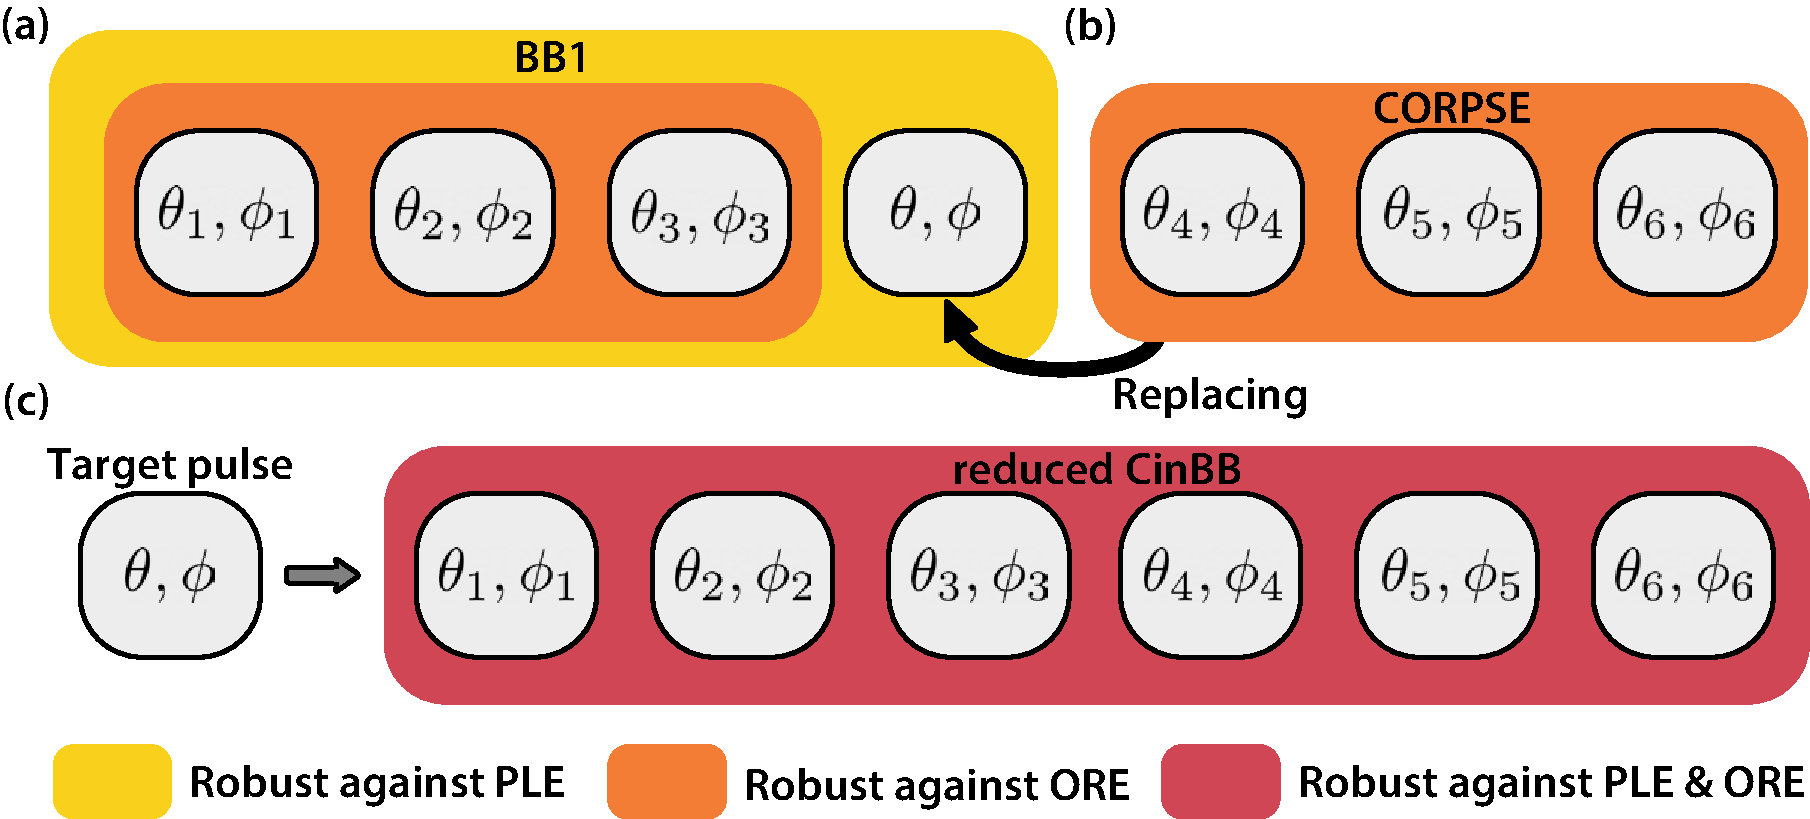
\includegraphics[width=\linewidth]{figs/SI_Fig_3.pdf}
    \caption{\textbf{Schematic construction of the six‐pulse \textit{r}CinBB composite pulse sequence.}
             (a) Four‐pulse BB1 outer sequence cancels PLE.
             (b) Three‐pulse CORPSE block cancels ORE and is REP‐PLE.
             (c) Substituting only the fourth BB1 rotation yields the
             six‐pulse rCinBB, first‐order robust to both PLE and ORE.}
    \label{fig:schematic_rCinBB}
  \end{figure}

\begingroup
  % Rename table numbering to have "S" prefix and reset counter
  \renewcommand{\thetable}{S\arabic{table}}

  \begin{table}
    \centering
    \begin{tabular}{|>{\centering\arraybackslash}p{0.15\textwidth}|
                    >{\centering\arraybackslash}p{0.15\textwidth}|}
      \hline
      $\theta_1 = \pi$                          & $\phi_1 = \phi + s$   \\[1ex]
      $\theta_2 = 2\pi$                        & $\phi_2 = \phi - 2\,s$ \\[1ex]
      $\theta_3 = \pi$                          & $\phi_3 = \phi + s$   \\[1ex]
      $\theta_4 = 2\pi + \tfrac{\theta}{2} - k$ & $\phi_4 = \phi$       \\[1ex]
      $\theta_5 = 2\pi - 2\,k$                  & $\phi_5 = \phi + \pi$ \\[1ex]
      $\theta_6 = \tfrac{\theta}{2} - k$        & $\phi_6 = \phi$       \\ \hline
      \multicolumn{2}{|c|}{%
        \begin{tabular}{c}
          $k = \arcsin\!\displaystyle\Bigl(\tfrac{\sin(\theta/2)}{2}\Bigr)$ \\[0.75ex]
          $s = \arccos\!\displaystyle\Bigl(-\tfrac{\theta}{4\pi}\Bigr)$
        \end{tabular}
      } \\ \hline
    \end{tabular}
    \caption{\textbf{Rotation parameters for the six-pulse rCinBB sequence.} The angles $\theta_i$ and phases $\phi_i$ define the elementary rotations $R(\theta_i,\phi_i)$ that compose the target gate $\hat{\mathcal{U}}_{\mathrm{ideal}}(\theta,\phi)$.}
    \label{tab:S2_theta_phi_CCCP}
  \end{table}
\endgroup

\subsection{SAFE-GRAPE Parameters}

Table \ref{tab:GRAPE_parameters} contains the parameters for the SAFE-GRAPE algorithm (adapted from \cite{khaneja_optimal_2005}) used in the main text. The set of trainable parameters $\{t_i , \phi_i \}_{i\in [1...N_p]}$ is initialized based on the rCinBB pulse sequence. All $t_i$ are set equal to the fraction of the rCinBB total pulse duration for chosen $\Omega$ over the number of time-bins $N_p$. Each $\phi_i$ is assigned the corresponding rCinBB phase $\in\{\phi_1, ...,\phi_6\}$ for time-bin $i$.  

\begingroup
    % Rename table numbering to have "S" prefix and reset counter
    \renewcommand{\thetable}{S\arabic{table}}
    \begin{table}[]
        \begin{tabular}{|c|c|c|c|}
        \hline
        \textbf{General}   & \textbf{\begin{tabular}[c]{@{}c@{}}Discretised composite\\[-1ex] search space\end{tabular}} & \textbf{\begin{tabular}[c]{@{}c@{}}Gaussian\\[-1ex] weight factor\end{tabular}} & \textbf{\begin{tabular}[c]{@{}c@{}}Sigmoid\\[-1ex] reparametrization\end{tabular}} \\ \hline
        $\theta=\pi$       & $N_{\epsilon} = N_f=11$         & $\mathcal{N}=1.90$                & $t_{min}=10^{-9}$ s                \\
        $\phi=0$           & $\epsilon_{min} = f_{min}=-0.3$ & $\bar{\epsilon}=\bar{f}=0$        & $t_{max}=10^{-8}$ s                \\
        $\Omega=200$ Mrad/s & $\epsilon_{max} = f_{max}=0.3$  & $\sigma_{\epsilon}=\sigma_f=0.22$ &                                    \\
        $N_p=100$          &                                 &                                   &                                    \\ \hline
        \end{tabular}
        \caption{\textbf{SAFE-GRAPE on rCinBB optimization parameters}}
        \label{tab:GRAPE_parameters}
    \end{table}

\subsection{Bandwidth Aware SAFE-GRAPE}
\label{sec_bandwidthawaresafe-grape}
\rev{In this section we show how it is possible to take experimental hardware constraints (maximum bandwidth $BW_{max}$ and Rabi drive strength $\Omega_{max}$) into account when finding the optimal control pulse sequence. Bandwidth Aware SAFE-GRAPE optimizes an I/Q control drive. It takes additional inputs $BW_{max}$, $\Omega_{max}$ and oversampling factor $N_{os}$. The pulse sequence consists of $N_p$ training segments, such that the set of trainable parameters is given by $\{I_i , Q_i \}_{i\in [1...N_p]}$. In order to enforce the bandwidth constraint, the control pulse is divided into sections of time $\Delta t=\frac{1}{2*BW_{max}*N_{os}}$ such that the Nyquist frequency is $N_{os}BW_{max}$. Each of these segments represents a pulse $\hat{\mathcal{U}}_{\epsilon , f}^{\text{real}}(I, Q)$.}

\begin{align*}
    \hat{\mathcal{U}}_{\epsilon , f}^{\text{real}}(I, Q) =  \exp{-i\frac{\Omega_{max}\Delta t}{2} [ (1+\epsilon_i)(I \hat{\sigma}_{x,i} + Q\hat{\sigma}_{y,i}) - i f_i \hat{\sigma}_{z,i} ] }
\end{align*}

\rev{The number of time steps $N_t$ is defined as the integer multiple of training segments $N_p$ that matches closest the total pulse duration $T_{pulse}=N_t\Delta_t$ with the duration of the initial pulse for a given Rabi drive strength. $N_t=N_{us}N_p$ with upsampling factor $N_{us}$. The initial guess for $I$ and $Q$ are based on the rCinBB composite pulse sequence. The complete control sequence is given by $\prod_{i=1}^{N_t}\hat{\mathcal{U}}_{\epsilon , f}^{\text{real}}(I'_i, Q'_i)$. Here $\{I'_i , Q'_i \}_{i\in [1...N_t]}$ are defined using the following three-step proces. First, $\{I_i , Q_i \}_{i\in [1...N_p]}$ is upsampled with factor $N_{us}$. Second, these parameters are sent through a Gaussian low-pass filter. This is done by convolution with a Gaussian kernel $g[n]=\frac{1}{\mathcal{N}_{kernel}}\exp{-\frac{n^2}{\sigma^2}}$, where $\sigma=\frac{\sqrt{\ln2}}{2\pi BW_{max}\Delta t}$ is chosen such that the bandwidth of the Gaussian filter is at $BW_{max}$. Third, if the amplitude $\sqrt{I_i^2 + Q_i^2}$ is larger than 1, we scale $I_i$ and $Q_i$ with a factor $\frac{1}{\sqrt{I_i^2 + Q_i^2}}$, i.e. we clip the amplitude at 1 so that we never have to drive the system stronger than $\Omega_{max}$. This results in the following definition of the total loss function $\mathcal{L}$:}


\begin{align}
\label{eq_lossfunction}
    \mathcal{L} = \sum_{(\epsilon , f) \in \boldsymbol{\Omega^*}} \underbrace{ \left[ 1 - \frac{1}{2}\text{Tr}\left[ \left( \hat{\mathcal{U}}^{\text{ideal}}(\theta,\phi) \right)^\dagger \prod_{i=1}^{N_t} \hat{\mathcal{U}}_{\epsilon , f}^{\text{real}}(I'_i, Q'_i) \right] \right] }_{1-\overline{\mathcal{F}}(\epsilon,f)} \mathcal{W}(\epsilon,f) % + \mathcal{L}_{p}
\end{align}


\rev{An example is shown in figure \ref{fig:BandwidthAwareSAFEGRAPE}. The optimization reduces the adapted loss function $\mathcal{L}$ from 108.69 to 0.18. For comparison, the standard SAFE-GRAPE algorithm from figure \ref{fig:GRAPE} reduces the loss function from 19.18 to 0.18. So we are able to recover a similar level of error mitigation on the same composite search space. Note that the loss function is different for both initial pulse sequences, because the bandwidth constraint also affects the initial pulse sequence.}



\begin{figure*}
    \centering
    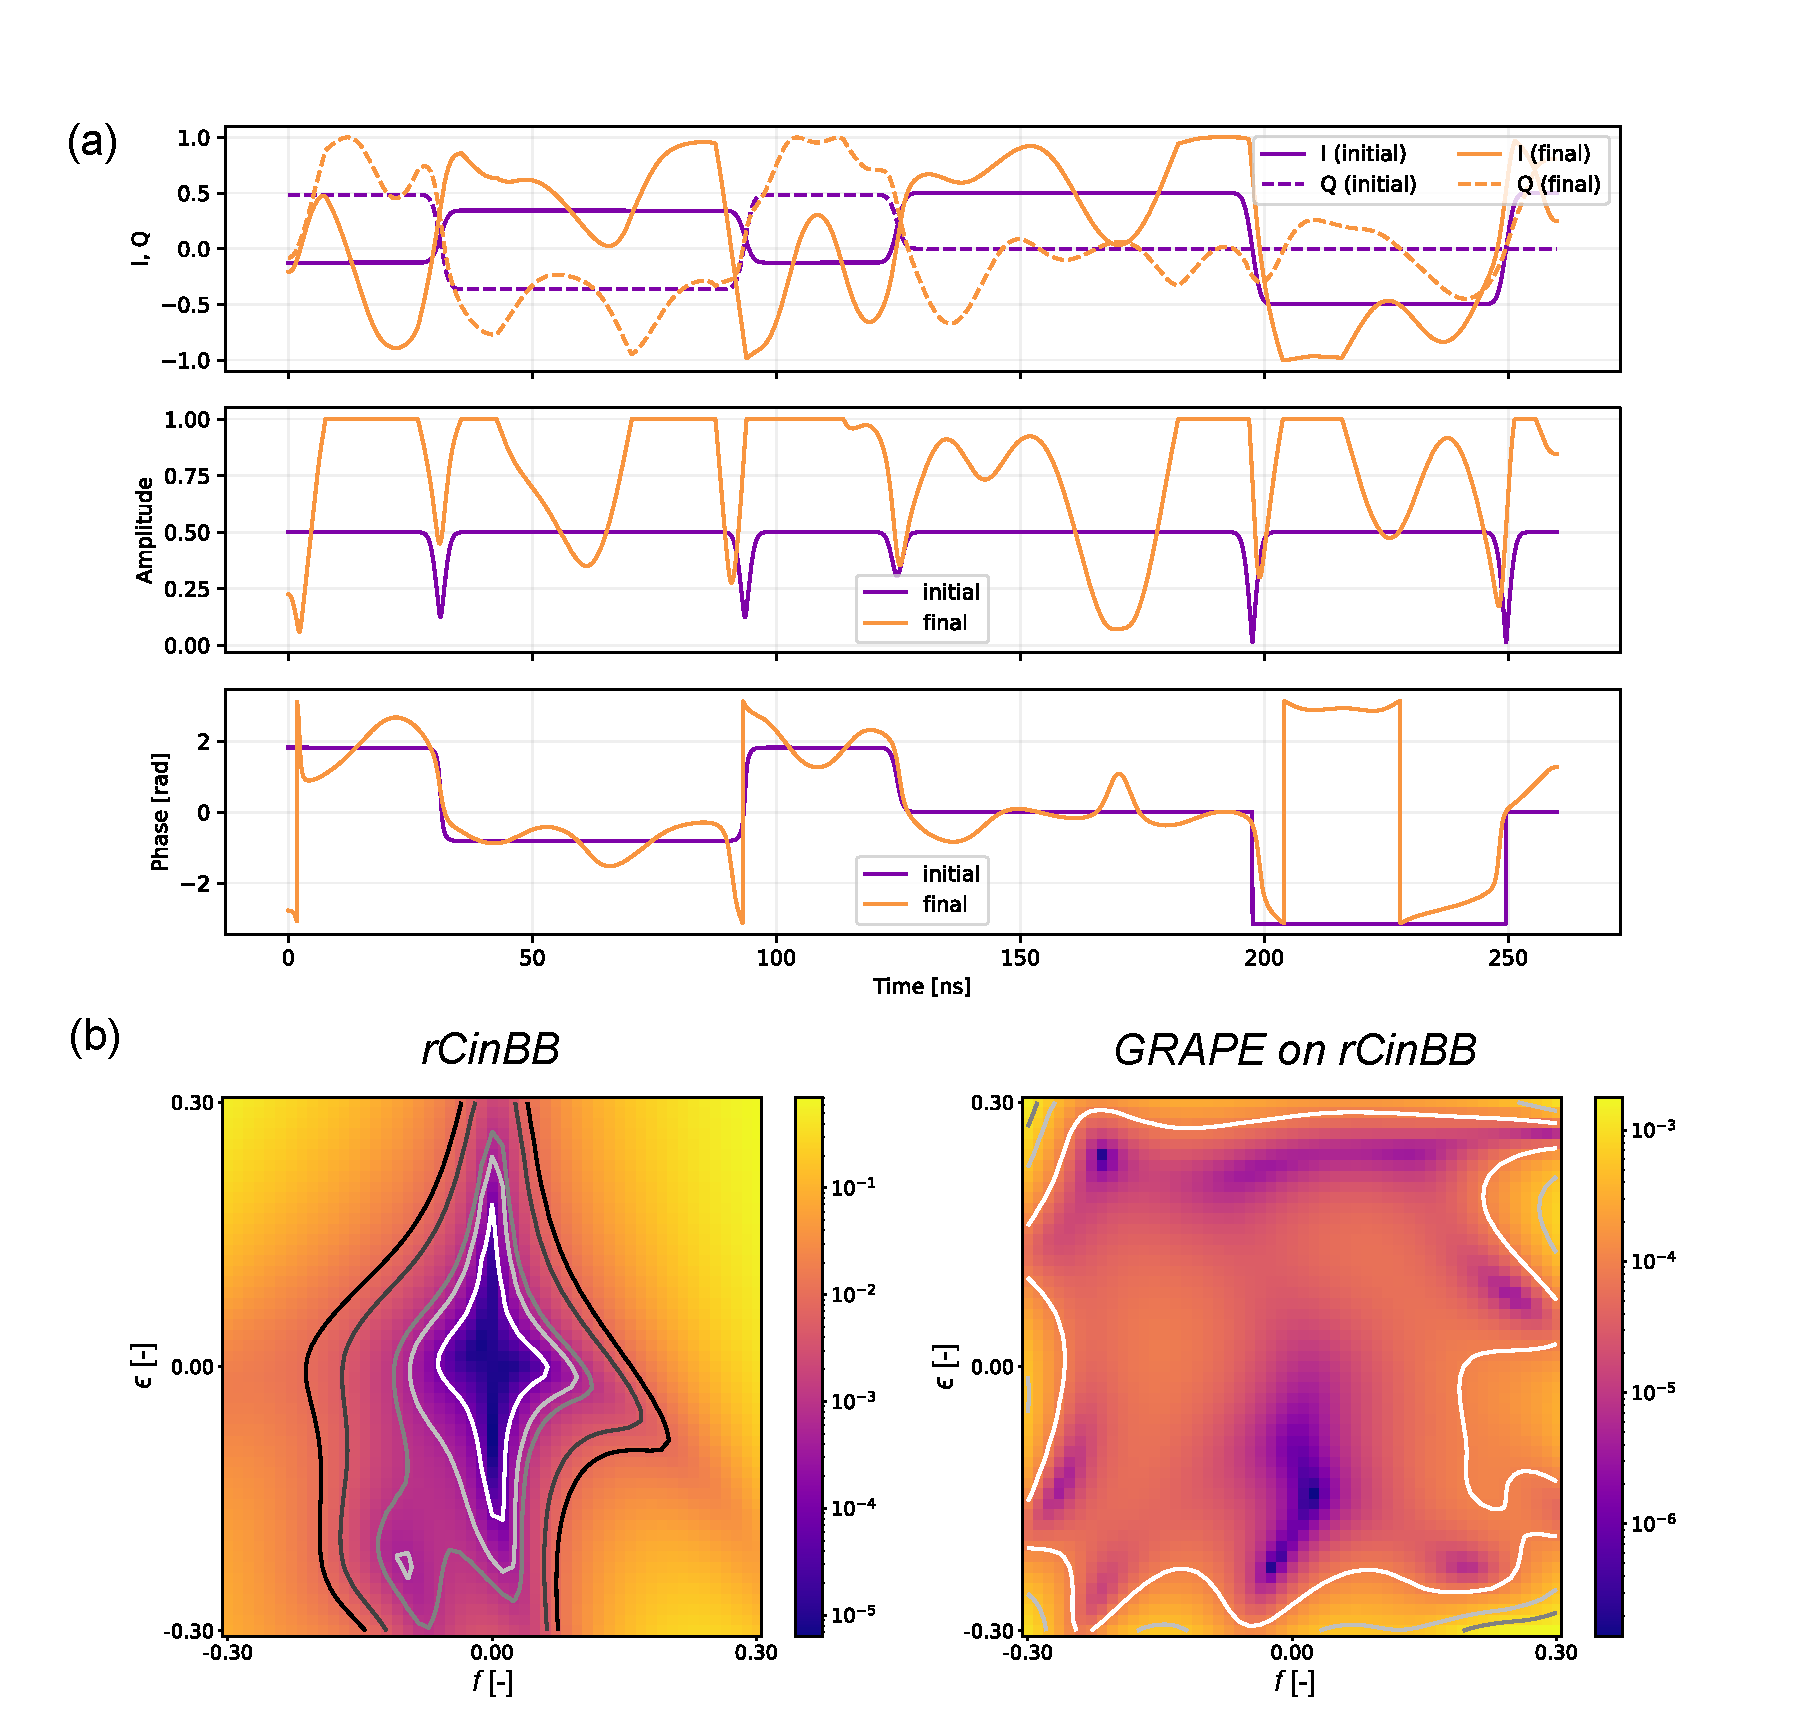
\includegraphics[width=\linewidth]{figs/BandwidthAwareSAFEGRAPE.pdf}
    \caption{\rev{\textbf{Bandwidth Aware SAFE-GRAPE. (a)} $I,Q$ parameters before and after GRAPE optimization with bandwidth constraint $BW_{max}=100$ MHz and amplitude constraint $\Omega_{max}=200$ Mrad/s. Oversampling factor $N_{os}=50$ is used. From $I,Q$ it is possible to calculate the amplitude (normalized to $\Omega_{max}$) $\sqrt{I^2+Q^2}$ and phase atan2$(Q,I)$. \textbf{(b)} Infidelity map of the composite pulse sequence before (left) and after (right) GRAPE optimization. Contours denote infidelities of $10^{-4}, 5\times10^{-4}, 10^{-3}, 5\times10^{-3}$ and $ 10^{-2}$, increasing from white to black. Note that both plots have their own color bar.}}
    \label{fig:BandwidthAwareSAFEGRAPE}
\end{figure*}

\section{Fidelity Calculation}
In order to estimate the fidelity of the links, we divide the process into four steps:\\
(A) Single-Photon Entanglement Protocol \cite{Hermans_2023}\\
(B-D) Dynamical Decoupling Sequence as a Dephasing Channel \cite{PhysRev.94.630, meiboom_modified_1958}\\
(E) Composing the Entanglement Protocol with Dynamical Decoupling\\
(F) Including the thermal budget\\

\begin{figure*}
    \centering
    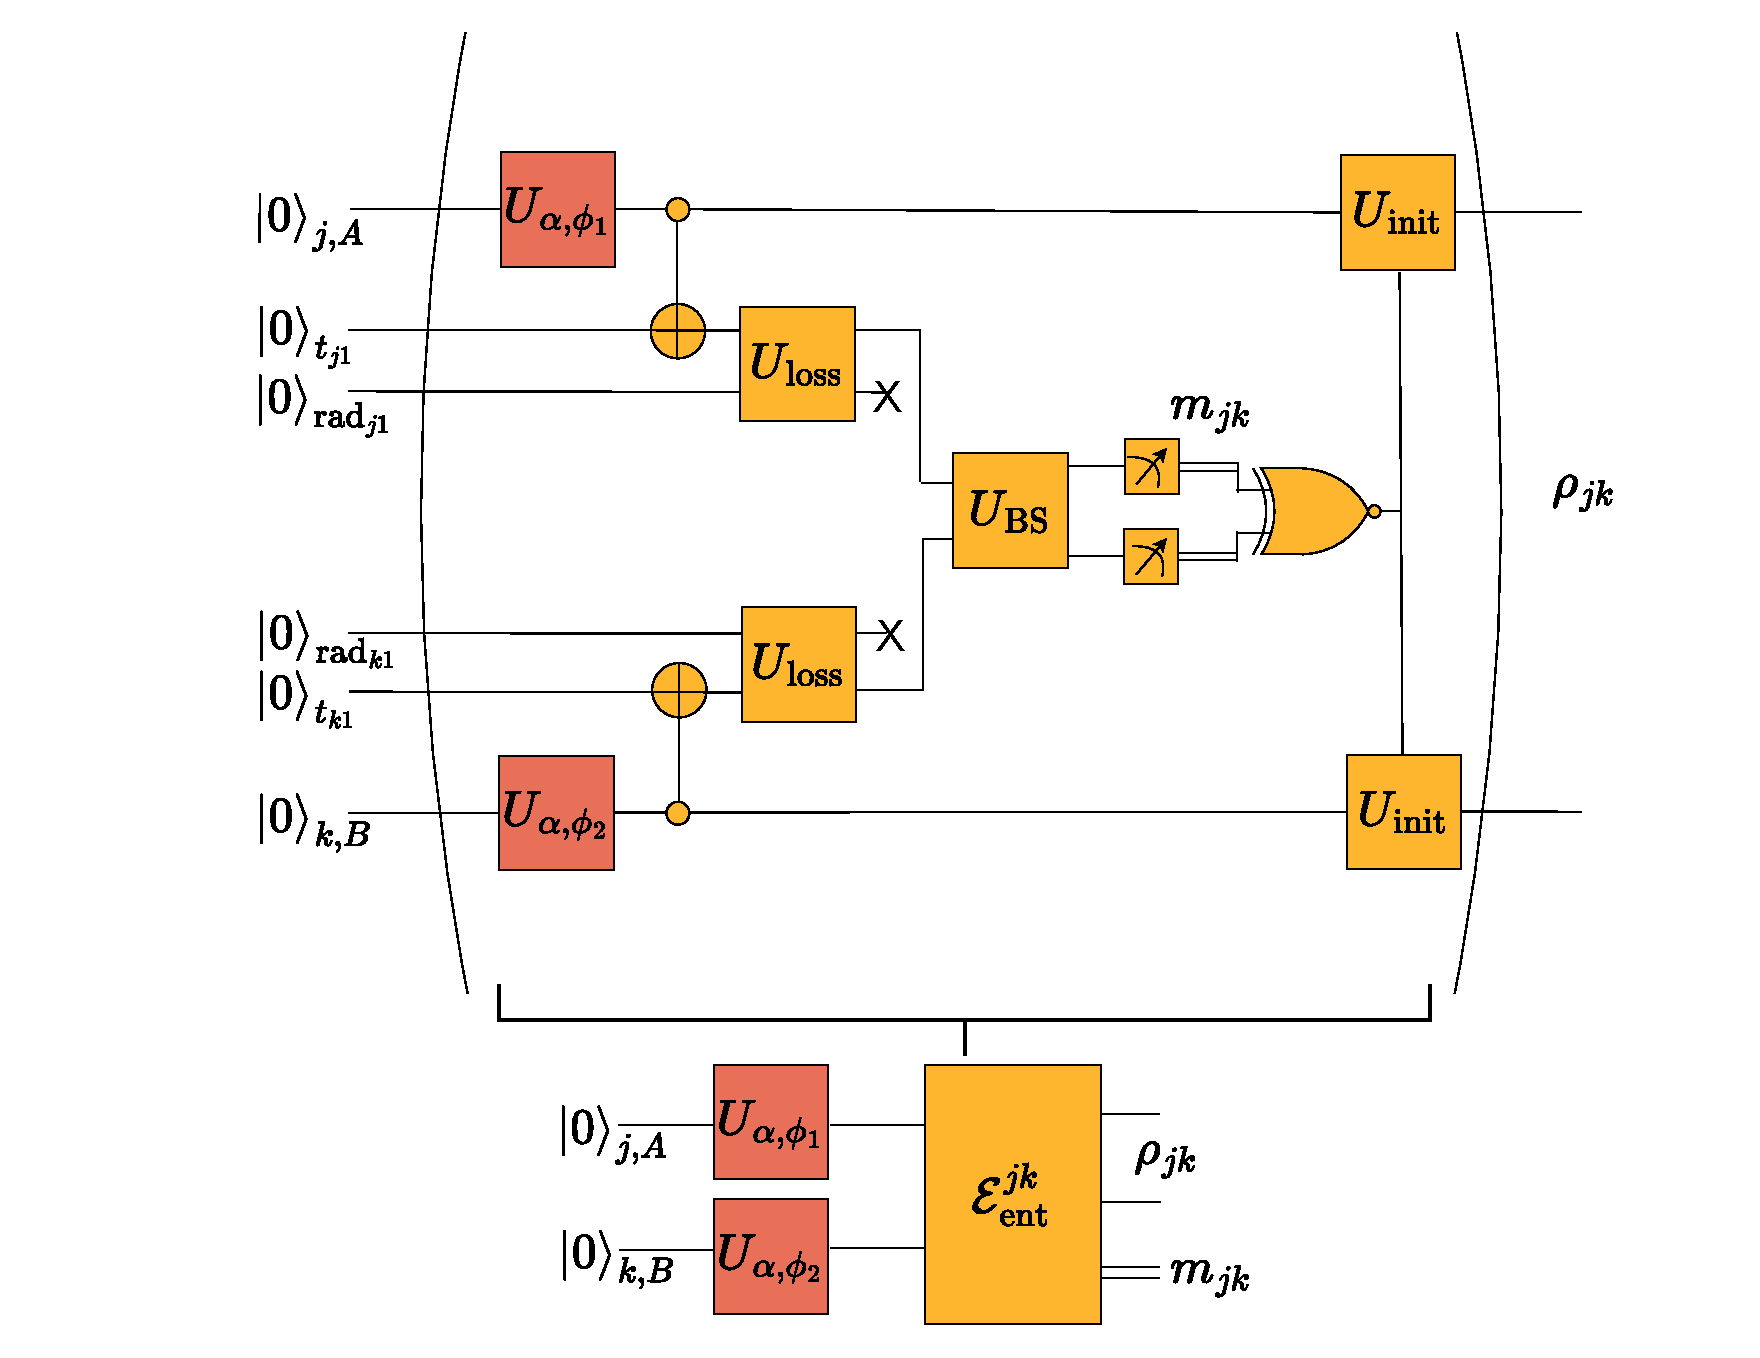
\includegraphics[width=0.9\linewidth]{figs/SI_Fig_4.pdf}
    \caption{\textbf{Single-Photon Entanglement Protocol.} Quantum Circuit Representation to perform remote entanglement between spin qubits $\ket{0}_{j,A}$ and $\ket{0}_{k,B}$. $\ket{0}_{t}$ and $\ket{0}_{\text{rad}}$ are the vacuum modes for the time-bin and radiative mode respectively. Inverted CNOT is physically realized by laser based spin selective excitation of the spin ground states. Following are the representation of the blocks - $U_{\alpha,\phi}$: Initialization unitary, $U_{\text{loss}}$: Loss channel, $U_{\text{BS}}$: Beam Splitter, $U_{\text{init}}$: measurement controlled laser based spin initialization. $m_{jk}$ is a two bit click result, where 0(1) means absence (presence) of detector click.}
    \label{fig:SPE}
\end{figure*}

\subsection{Single-Photon Entanglement Protocol}
Fig.~\ref{fig:SPE} shows the quantum circuit representation \cite{Nielsen_Chuang_2010} of the N-cycle single-photon entanglement protocol. We start the protocol between qubits $j$ and $k$, from system A and B respectively, in their respective ground states $\ket{0}_{j,A}$ and $\ket{0}_{k,B}$. The states $\ket{0}_{t_{jm}}$ and $\ket{0}_{t_{km}}$ represents the zero photon in the time-bins $t_{jm}$ and $t_{km}$ respectively, for the $m^{\text{th}}$ attempt. Similarly, the states $\ket{0}_{\text{rad}_{jm}}$ and $\ket{0}_{\text{rad}_{km}}$ represents the zero radiative photons for the qubits $j$ and $k$ respectively, for the $m^{\text{th}}$ attempt. Thus, the initial state at the first attempt is given by:
\begin{equation}
    \ket{\psi}_{in} = \ket{0}_{j,A}\otimes\ket{0}_{t_{j1}}\otimes\ket{0}_{\text{rad}_{j1}}\otimes\ket{0}_{k,B}\otimes\ket{0}_{t_{k1}}\otimes\ket{0}_{\text{rad}_{k1}}
\end{equation}
We use the following two compact notations:
\begin{subequations}
\begin{align}
    \ket{\psi}_{in} &= \ket{00}_{jk}\otimes\ket{00}_{t}\otimes \ket{00}_{\text{rad}}\\
    &= \ket{000}_{j,t,\text{rad}}\otimes\ket{000}_{k,t,\text{rad}}
\end{align}    
\end{subequations}
where in the first notation: the three different Hilbert spaces correspond to two qubits, two time bins, and two radiative modes respectively and in the second notation: the two different Hilbert spaces correspond to the two systems. We apply the arbitrary unitary $U_{\alpha,\phi}$ on $\ket{\psi}_{in}$, whose action on the ground state is defined as:
\begin{equation}
    U_{\alpha,\phi}:\ket{0}_{j}\to \sqrt{\alpha}\ket{0}_{j} + \text{e}^{i\phi}\sqrt{1-\alpha}\ket{1}_{j}
\end{equation}
This results in the following:
\begin{subequations}
\begin{align}
     &(U_{\alpha,\phi_{1}}\otimes U_{\alpha,\phi_{2}})\ket{\psi}_{in} \nonumber \\
     &= (\sqrt{\alpha}\ket{0}_{j} + \text{e}^{i\phi_{1}}\sqrt{1-\alpha}\ket{1}_{j})\otimes(\sqrt{\alpha}\ket{0}_{k} + \text{e}^{i\phi_{2}}\sqrt{1-\alpha}\ket{1}_{k})\otimes\ket{00}_{t}\otimes\ket{00}_{\text{rad}}\\
     &= (\sqrt{\alpha}\ket{000}_{j,t,\text{rad}} + \text{e}^{i\phi_{1}}\sqrt{1-\alpha}\ket{100}_{j,t,\text{rad}})\otimes (\sqrt{\alpha}\ket{000}_{k,t,\text{rad}} + \text{e}^{i\phi_{2}}\sqrt{1-\alpha}\ket{100}_{k,t,\text{rad}})
\end{align}
\end{subequations}
Next, we apply a CNOT gate on the two systems A and B. This corresponds to laser mediated state selective excitation.  We call the resulting state $\ket{\psi}_{2}$. Each CNOT acts between the spin qubit and time-bin qubit, which gives the following:
\begin{subequations}
    \begin{align}
        \ket{\psi}_{2} =& (\text{CNOT}_{A})\otimes (\text{CNOT}_{B})(U_{\alpha,\phi_{1}}\otimes U_{\alpha,\phi_{2}})\ket{\psi}_{in}\\
        =& (\text{CNOT}_{A})(\sqrt{\alpha}\ket{000}_{j,t,\text{rad}} + \text{e}^{i\phi_{1}}\sqrt{1-\alpha}\ket{100}_{j,t,\text{rad}})\nonumber\\
        &\otimes (\text{CNOT}_{B})(\sqrt{\alpha}\ket{000}_{k,t,\text{rad}} + \text{e}^{i\phi_{2}}\sqrt{1-\alpha}\ket{100}_{k,t,\text{rad}})\\
        =& (\sqrt{\alpha}\ket{010}_{j,t,\text{rad}} + \text{e}^{i\phi_{1}}\sqrt{1-\alpha}\ket{100}_{j,t,\text{rad}})\nonumber\\
        &\otimes(\sqrt{\alpha}\ket{010}_{k,t,\text{rad}} + \text{e}^{i\phi_{2}}\sqrt{1-\alpha}\ket{100}_{k,t,\text{rad}})
    \end{align}
\end{subequations}
Next, the photon loss \(1-\eta\) is modeled using a beamsplitter model acting on the qubits labeled $t$ and $\text{rad}$ as follows:
\begin{subequations}
\begin{align}
    U_{\text{loss}}\ket{00}_{t,\text{rad}} &= \ket{00}_{t,\text{rad}}\\
     U_{\text{loss}}\ket{10}_{t,\text{rad}} &= \sqrt{\eta}\ket{10}_{t,\text{rad}} + \sqrt{1-\eta}\ket{01}_{t,\text{rad}}
\end{align}
\end{subequations}
Let $\ket{\psi}_{3}=U_{\text{loss,A}}\otimes U_{\text{loss,B}}\ket{\psi}_2$. With the beamsplitter model defined above, this gives:
\begin{subequations}
    \begin{align}
        \ket{\psi}_{3}=& U_{\text{loss,A}}(\sqrt{\alpha}\ket{010}_{j,t,\text{rad}} + \text{e}^{i\phi_{1}}\sqrt{1-\alpha}\ket{100}_{j,t,\text{rad}})\nonumber\\
        &\otimes U_{\text{loss,B}}(\sqrt{\alpha}\ket{010}_{k,t,\text{rad}} + \text{e}^{i\phi_{2}}\sqrt{1-\alpha}\ket{100}_{k,t,\text{rad}})\\
        =& (\sqrt{\alpha}\ket{0}_{j}U_{\text{loss,A}}\ket{10}_{t,\text{rad}} + \text{e}^{i\phi_{1}}\sqrt{1-\alpha}\ket{1}_{j}U_{\text{loss,A}}\ket{00}_{t,\text{rad}})\nonumber\\
        &\otimes(\sqrt{\alpha}\ket{0}_{k}U_{\text{loss,B}}\ket{10}_{t,\text{rad}} + \text{e}^{i\phi_{2}}\sqrt{1-\alpha}\ket{1}_{k}U_{\text{loss,B}}\ket{00}_{t,\text{rad}}) \\
        =& [\sqrt{\alpha}\ket{0}_{j}(\sqrt{\eta}\ket{10}_{t,\text{rad}} + \sqrt{1-\eta}\ket{01}_{t,\text{rad}}) + \text{e}^{i\phi_{1}}\sqrt{1-\alpha}\ket{1}_{j}\ket{00}_{t,\text{rad}}]\nonumber\\
        &\otimes[\sqrt{\alpha}\ket{0}_{k}(\sqrt{\eta}\ket{10}_{t,\text{rad}} + \sqrt{1-\eta}\ket{01}_{t,\text{rad}}) + \text{e}^{i\phi_{2}}\sqrt{1-\alpha}\ket{1}_{k}\ket{00}_{t,\text{rad}}] \\
        =& (\sqrt{\alpha\eta}\ket{010}_{j,t,\text{rad}} + \sqrt{\alpha(1-\eta)}\ket{001}_{j,t,\text{rad}} + \text{e}^{i\phi_{1}}\sqrt{1-\alpha}\ket{100}_{j,t,\text{rad}}) \nonumber\\
        &\otimes (\sqrt{\alpha\eta}\ket{010}_{k,t,\text{rad}} + \sqrt{\alpha(1-\eta)}\ket{001}_{k,t,\text{rad}} + \text{e}^{i\phi_{2}}\sqrt{1-\alpha}\ket{100}_{k,t,\text{rad}})\\
        =& \alpha\eta\ket{0011}_{j,k,t,t}\ket{00}_{\text{rad}} + \alpha\sqrt{\eta(1-\eta)}\ket{0010}_{j,k,t,t}\ket{01}_{\text{rad}}\nonumber\\
        & + \text{e}^{i\phi_{2}}\sqrt{\eta\alpha(1-\alpha)}\ket{0110}_{j,k,t,t}\ket{00}_{\text{rad}} + \alpha\sqrt{\eta(1-\eta)}\ket{0001}_{j,k,t,t}\ket{10}_{\text{rad}}\nonumber\\
        & + \alpha(1-\eta)\ket{0000}_{j,k,t,t}\ket{11}_{\text{rad}}+ \text{e}^{i\phi_{2}}\sqrt{\alpha(1-\alpha)(1-\eta)}\ket{0100}_{j,k,t,t}\ket{10}_{\text{rad}}\nonumber\\
        & + \text{e}^{i\phi_{1}}\sqrt{\eta\alpha(1-\alpha)}\ket{1001}_{j,k,t,t}\ket{00}_{\text{rad}}+ \text{e}^{i\phi_{1}}\sqrt{\alpha(1-\alpha)(1-\eta)}\ket{1000}_{j,k,t,t}\ket{01}_{\text{rad}}\nonumber\\
        & + \text{e}^{i(\phi_{1}+\phi_{2})}(1-\alpha)\ket{1100}_{j,k,t,t}\ket{00}_{\text{rad}}
    \end{align}
\end{subequations}
We now trace over the radiative degree of freedom:
\begin{subequations}
    \begin{align}
        \rho_{4} =& \text{Tr}_{\text{rad}}(\ket{\psi}_{3}\bra{\psi}_{3})\\
        =& \bra{00}_{\text{rad}}\ket{\psi}_{3}\bra{\psi}_{3}\ket{00}_{\text{rad}} + \bra{01}_{\text{rad}}\ket{\psi}_{3}\bra{\psi}_{3}\ket{01}_{\text{rad}}\nonumber\\
        &+ \bra{10}_{\text{rad}}\ket{\psi}_{3}\bra{\psi}_{3}\ket{10}_{\text{rad}} + \bra{11}_{\text{rad}}\ket{\psi}_{3}\bra{\psi}_{3}\ket{11}_{\text{rad}}
    \end{align}
\end{subequations}
From above equations, we get the following terms (here we omit subscript $j,k,t,t$):
\begin{subequations}
    \begin{align}
        \bra{00}_\text{rad}\ket{\psi}_{3} &= \alpha\eta\ket{0011} + \text{e}^{i\phi_{2}}\sqrt{\eta\alpha(1-\alpha)}\ket{0110} + \text{e}^{i\phi_{1}}\sqrt{\eta\alpha(1-\alpha)}\ket{1001} + \text{e}^{i(\phi_{1}+\phi_{2})}(1-\alpha)\ket{1100}\\
        \bra{01}_\text{rad}\ket{\psi}_{3} &=
        \alpha\sqrt{\eta(1-\eta)}\ket{0010} + \text{e}^{i\phi_{1}}\sqrt{\alpha(1-\alpha)(1-\eta)}\ket{1000}\\
        \bra{10}_\text{rad}\ket{\psi}_{3} &= \alpha\sqrt{\eta(1-\eta)}\ket{0001} + \text{e}^{i\phi_{2}}\sqrt{\alpha(1-\alpha)(1-\eta)}\ket{0100}\\
        \bra{11}_\text{rad}\ket{\psi}_{3} &=
        \alpha(1-\eta)\ket{0000}
    \end{align}
\end{subequations}
We use the following short-hand notation:
\begin{equation}
        \ket{c_{d(j)}}\equiv\ket{j}
\end{equation}
where $j$ is a 4-bit binary number, and $d(j)$ is decimal representation of $j$. We can rewrite Eq.12 as follows:
\begin{subequations}
    \begin{align}
        \bra{00}_\text{rad}\ket{\psi}_{3} =& \alpha\eta\ket{c_{3}} + \text{e}^{i\phi_{2}}\sqrt{\eta\alpha(1-\alpha)}\ket{c_{6}} + \text{e}^{i\phi_{1}}\sqrt{\eta\alpha(1-\alpha)}\ket{c_{9}} \nonumber\\
        &+ \text{e}^{i(\phi_{1}+\phi_{2})}(1-\alpha)\ket{c_{12}}\\
        \bra{01}_\text{rad}\ket{\psi}_{3} =&
        \alpha\sqrt{\eta(1-\eta)}\ket{c_{2}} + \text{e}^{i\phi_{1}}\sqrt{\alpha(1-\alpha)(1-\eta)}\ket{c_{8}}\\
        \bra{10}_\text{rad}\ket{\psi}_{3} =& \alpha\sqrt{\eta(1-\eta)}\ket{c_{1}} + \text{e}^{i\phi_{2}}\sqrt{\alpha(1-\alpha)(1-\eta)}\ket{c_{4}}\\
        \bra{11}_\text{rad}\ket{\psi}_{3} =&
        \alpha(1-\eta)\ket{c_{0}}
    \end{align}
\end{subequations}
Using the above notations, and plugging in all the terms in Eq.11, we get the following:
\begin{align}
    \rho_{4} =& \alpha^2\eta^2\ket{c_3}\bra{c_3} + \eta\alpha(1-\alpha)\ket{c_6}\bra{c_6} + \eta\alpha(1-\alpha)\ket{c_9}\bra{c_9} + (1-\alpha)^2\ket{c_{12}}\bra{c_{12}}\nonumber\\
    &+ \sqrt{\alpha^3\eta^{3}(1-\alpha)}(\text{e}^{-i\phi_{2}}\ket{c_3}\bra{c_6} + \text{e}^{i\phi_{2}}\ket{c_6}\bra{c_3}) \nonumber\\
    &+ \sqrt{\alpha^3\eta^{3}(1-\alpha)}(\text{e}^{-i\phi_{1}}\ket{c_3}\bra{c_9} + \text{e}^{i\phi_{1}}\ket{c_9}\bra{c_3})\nonumber\\
    &+ \eta\alpha(1-\alpha)(\text{e}^{i(\phi_{2}-\phi_{1})}\ket{c_6}\bra{c_9} + \text{e}^{i(\phi_{1}-\phi_{2})}\ket{c_9}\bra{c_6}) \nonumber\\
    &+ \sqrt{\eta\alpha(1-\alpha)^3}(\text{e}^{-i\phi_{1}}\ket{c_6}\bra{c_{12}} + \text{e}^{i\phi_{1}}\ket{c_{12}}\bra{c_6})\nonumber\\
    &+ \sqrt{\eta\alpha(1-\alpha)^3}(\text{e}^{-i\phi_{2}}\ket{c_9}\bra{c_{12}} + \text{e}^{i\phi_{2}}\ket{c_{12}}\bra{c_9}) \nonumber\\
    &+ \eta\alpha(1-\alpha)(\text{e}^{-i(\phi_{1}+\phi_{2})}\ket{c_3}\bra{c_{12}} + \text{e}^{i(\phi_{1}+\phi_{2})}\ket{c_{12}}\bra{c_3})\nonumber\\
    &+ \alpha^2\eta(1-\eta)\ket{c_2}\bra{c_2} + \alpha(1-\alpha)(1-\eta)\ket{c_8}\bra{c_8} \nonumber\\
    &+ \sqrt{\alpha^3\eta(1-\alpha)(1-\eta)^2}(\text{e}^{-i\phi_{1}}\ket{c_2}\bra{c_8} + \text{e}^{i\phi_{1}}\ket{c_8}\bra{c_2})\nonumber\\
    &+ \alpha^2\eta(1-\eta)\ket{c_1}\bra{c_1} + \alpha(1-\alpha)(1-\eta)\ket{c_4}\bra{c_4} \nonumber\\
    &+ \sqrt{\alpha^3\eta(1-\alpha)(1-\eta)^2}(\text{e}^{-i\phi_{2}}\ket{c_1}\bra{c_4} + \text{e}^{i\phi_{2}}\ket{c_4}\bra{c_1})\nonumber\\
    &+ \alpha^2(1-\eta)^2\ket{c_0}\bra{c_0}
\end{align}
After this stage, the two time bin qubits experience the following transformation due to the beam splitter:
\begin{subequations}
    \begin{align}
        &U_{\text{BS}}:\ket{00}^{A,B}_{t,t}\to \ket{00}^{C,D}_{t,t}\\
        &U_{\text{BS}}:\ket{01}^{A,B}_{t,t}\to \frac{\ket{10}^{C,D}_{t,t}-\ket{01}^{C,D}_{t,t}}{\sqrt{2}}\\
        &U_{\text{BS}}:\ket{10}^{A,B}_{t,t}\to \frac{\ket{10}^{C,D}_{t,t}+\ket{01}^{C,D}_{t,t}}{\sqrt{2}}\\
        &U_{\text{BS}}:\ket{11}^{A,B}_{t,t}\to \frac{\ket{20}^{C,D}_{t,t}-\ket{02}^{C,D}_{t,t}}{2}\\
        &(\text{assuming perfect indistinguishability of the two incoming photons})\nonumber
    \end{align}
\end{subequations}
Here, $A, B$ are the incoming ports and $C,D$ are the outgoing ports of the beamsplitter. The state after the beamsplitter is:
\begin{equation}
    \rho_{5} = U_{\text{BS}}\rho_{4}U_{\text{BS}}^{\dagger}
\end{equation}
We define the following measurement operators for getting statistics of clicks:
\begin{subequations}
    \begin{align}
        \text{M}_{C1} &= \ket{10}^{C,D}_{t,t} \bra{10}^{C,D}_{t,t}: \text{single click in port C and no click in port D}\\
        \text{M}_{D1} &= \ket{01}^{C,D}_{t,t} \bra{01}^{C,D}_{t,t}: \text{single click in port D and no click in port C}\\
        \text{M}_{0} &= \ket{00}^{C,D}_{t,t} \bra{00 }^{C,D}_{t,t}: \text{no clicks in both ports}
    \end{align}
\end{subequations}
The probabilities for the events above are given as follows:
\begin{subequations}
    \begin{align}
        p_{C1} &= \text{Tr}(M_{C1}\rho_{5}) = \text{Tr}(\bra{10}^{C,D}_{t,t}\rho_{5}\ket{10}^{C,D}_{t,t}) = \text{Tr}(\bra{10}^{C,D}_{t,t}U_{\text{BS}}\rho_{4}U_{\text{BS}}^{\dagger}\ket{10}^{C,D}_{t,t})\\
        &= \text{Tr}\bigg(\frac{\bra{10}^{A,B}_{t,t}+\bra{01}^{A,B}_{t,t}}{\sqrt{2}} \rho_{4}        \frac{\ket{10}^{A,B}_{t,t}+\ket{01}^{A,B}_{t,t}}{\sqrt{2}} \bigg)\\
        &= \frac{ \text{Tr}(\bra{10}\rho_{4}\ket{10}) + \text{Tr}(\bra{10}\rho_{4}\ket{01}) + \text{Tr}(\bra{01}\rho_{4}\ket{10}) + \text{Tr}(\bra{01}\rho_{4}\ket{01}) }{2}
    \end{align}
\end{subequations}
Only the terms with $(c_{1}, c_{2}, c_{5}, c_{6}, c_{9}, c_{10}, c_{13}, c_{14})$ in $\rho_{4}$ lead to non-zero trace in the above expression. Let $\rho_{C1}$ be the density after the measurement $M_{C1}$. 
\begin{subequations}
    \begin{align}
        \rho_{C1} =&  \eta\alpha(1-\alpha)\ket{c_6}\bra{c_6} + \eta\alpha(1-\alpha)\ket{c_9}\bra{c_9} + \eta\alpha(1-\alpha)(\text{e}^{i(\phi_{2}-\phi_{1})}\ket{c_6}\bra{c_9} \nonumber\\
        &+ \text{e}^{i(\phi_{1}-\phi_{2})}\ket{c_9}\bra{c_6}) + \alpha^2\eta(1-\eta)\ket{c_2}\bra{c_2} + \alpha^2\eta(1-\eta)\ket{c_1}\bra{c_1}\\
        =& \frac{\eta\alpha(1-\alpha)}{2}\ket{01}_{j,k}\bra{01} + \frac{\eta\alpha(1-\alpha)}{2}\ket{10}_{j,k}\bra{10} + \frac{\eta\alpha(1-\alpha)}{2}\text{e}^{i(\phi_{2}-\phi_{1})}\ket{01}_{j,k}\bra{10}\nonumber\\
        &+ \frac{\eta\alpha(1-\alpha)}{2}\text{e}^{i(\phi_{1}-\phi_{2})}\ket{10}_{j,k}\bra{01} + \alpha^2\eta(1-\eta)\ket{00}_{j,k}\bra{00}\\
        =& \frac{\eta\alpha(1-\alpha)}{2}(\ket{01}_{j,k}\bra{01} + \ket{10}_{j,k}\bra{10} + \text{e}^{-i\Delta\phi}\ket{01}_{j,k}\bra{10} + \text{e}^{i\Delta\phi}\ket{10}_{j,k}\bra{01})\nonumber\\
        &+ \alpha^2\eta(1-\eta)\ket{00}_{j,k}\bra{00}\\
        =& \eta\alpha(1-\alpha)\ket{\Phi^{\Delta\phi}_{+}}\bra{\Phi^{{\Delta\phi}}_{+}}+ \alpha^2\eta(1-\eta)\ket{00}_{j,k}\bra{00}
    \end{align}
\end{subequations}
Here, $\ket{\Phi^{\Delta\phi}_{\pm}} = \frac{1}{\sqrt{2}}(\ket{01}_{j,k} \pm \text{e}^{i\Delta\phi}\ket{10}_{j,k})$, and $\Delta\phi = (\phi_{1}-\phi_{2})$. Hence we find:
\begin{equation}
    p_{C1} = \text{Tr}(\rho_{C1}) = p_{\text{click}} = 2\alpha\eta - 2\alpha^2\eta^2
\end{equation}
The normalized density matrix is given by:
\begin{align}
    \Tilde{\rho}_{C1} = \frac{1-\alpha}{1-\alpha\eta}\ket{\Phi^{\Delta\phi}_{+}}\bra{\Phi^{\Delta\phi}_{+}} + \frac{\alpha(1-\eta)}{1-\alpha\eta}\ket{00}_{j,k}\bra{00}
\end{align}
Analogously, we get the following expression for $\Tilde{\rho}_{D1}$:
\begin{align}
    \Tilde{\rho}_{D1} = \frac{1-\alpha}{1-\alpha\eta}\ket{\Phi^{\Delta\phi}_{-}}\bra{\Phi^{\Delta\phi}_{-}} + \frac{\alpha(1-\eta)}{1-\alpha\eta}\ket{00}_{j,k}\bra{00}
\end{align}
Thus, the fidelity of the heralded state is given by:
\begin{equation}
    F = \bra{\Phi^{\Delta\phi}_{+}}\Tilde{\rho}_{C1}\ket{\Phi^{\Delta\phi}_{+}}=\bra{\Phi^{\Delta\phi}_{-}}\Tilde{\rho}_{D1}\ket{\Phi^{\Delta\phi}_{-}} = F =\frac{1-\alpha}{1-\alpha\eta}
\end{equation}
In reality because of the dephasing in individual systems, phases of qubits in system A and B have noise contributions. Suppose for a measurement run, the phases are given by:
\begin{subequations}
    \begin{align}
        \Tilde{\phi}_{1} &= \phi_{1} + n_{\phi_{1}}\\
        \Tilde{\phi}_{2} &= \phi_{2} + n_{\phi_{2}}\\
        \Delta\Tilde{\phi} &= \Tilde{\phi}_{1}- \Tilde{\phi}_{2} = \Delta\phi + (n_{\phi_{1}}-n_{\phi_{2}}) = \Delta\phi + \Delta n_{\phi}
    \end{align}
\end{subequations}
Here, $n_{\phi_{1(2)}}$ is the random phase noise for a measurement run in system A(B). Let $\Tilde{\rho}_{C1,exp}$ be the density matrix that we expect experimentally, given by:
\begin{align}
    \Tilde{\rho}_{C1,exp} = \frac{1-\alpha}{1-\alpha\eta}\ket{\Phi^{\Delta\Tilde{\phi}}_{+}}\bra{\Phi^{\Delta\Tilde{\phi}}_{+}} + \frac{\alpha(1-\eta)}{1-\alpha\eta}\ket{00}_{j,k}\bra{00}
\end{align}
In that case, the fidelity we expect experimentally is given by:
\begin{subequations}
   \begin{align}
        F_{exp} &= \bra{\Phi^{\Delta\phi}_{+}}\Tilde{\rho}_{C1,exp}\ket{\Phi^{\Delta\phi}_{+}}=\bra{\Phi^{\Delta\phi}_{-}}\Tilde{\rho}_{D1,exp}\ket{\Phi^{\Delta\phi}_{-}}\\
        &= \text{cos}^{2}\bigg(\frac{\Delta n_{\phi}}{2}\bigg)\frac{1-\alpha}{1-\alpha\eta}
    \end{align} 
\end{subequations}
Similarly, the state we get after the measurement $M_{0}$ is given by:
\begin{subequations}
    \begin{align}
       \rho_{0} =& \bra{00}^{C,D}_{t,t}\rho_{5}\ket{00}^{C,D}_{t,t}\\ 
       =& (1-\alpha)^2\ket{11}_{j,k}\bra{11} + \alpha(1-\alpha)(1-\eta)(\ket{01}_{j,k}\bra{01} + \ket{10}_{j,k}\bra{10})\nonumber\\
       &+ \alpha^2(1-\eta)^2\ket{00}_{j,k}\bra{00}
    \end{align}
\end{subequations}
and the corresponding probability $p_0$ by:
\begin{equation}
    p_{0} = \text{Tr}(\rho_{0}) = (1-\alpha\eta)^2
\end{equation}
So the normalized density matrix becomes:
\begin{subequations}
    \begin{align}
        \Tilde{\rho}_{0} =& \frac{\rho_{0}}{\text{Tr}(\rho_{0})}\\
        =& \bigg(\frac{\alpha-\alpha\eta}{1-\alpha\eta}\bigg)^2\ket{00}_{j,k}\bra{00} + \bigg(\frac{1-\alpha}{1-\alpha\eta}\bigg)^2\ket{11}_{j,k}\bra{11}\nonumber\\
        &+ \frac{\alpha(1-\alpha)(1-\eta)}{(1-\alpha\eta)^2}\bigg(\ket{01}_{j,k}\bra{01} + \ket{10}_{j,k}\bra{10}\bigg)
    \end{align}
\end{subequations}
\begin{figure}
    \centering
    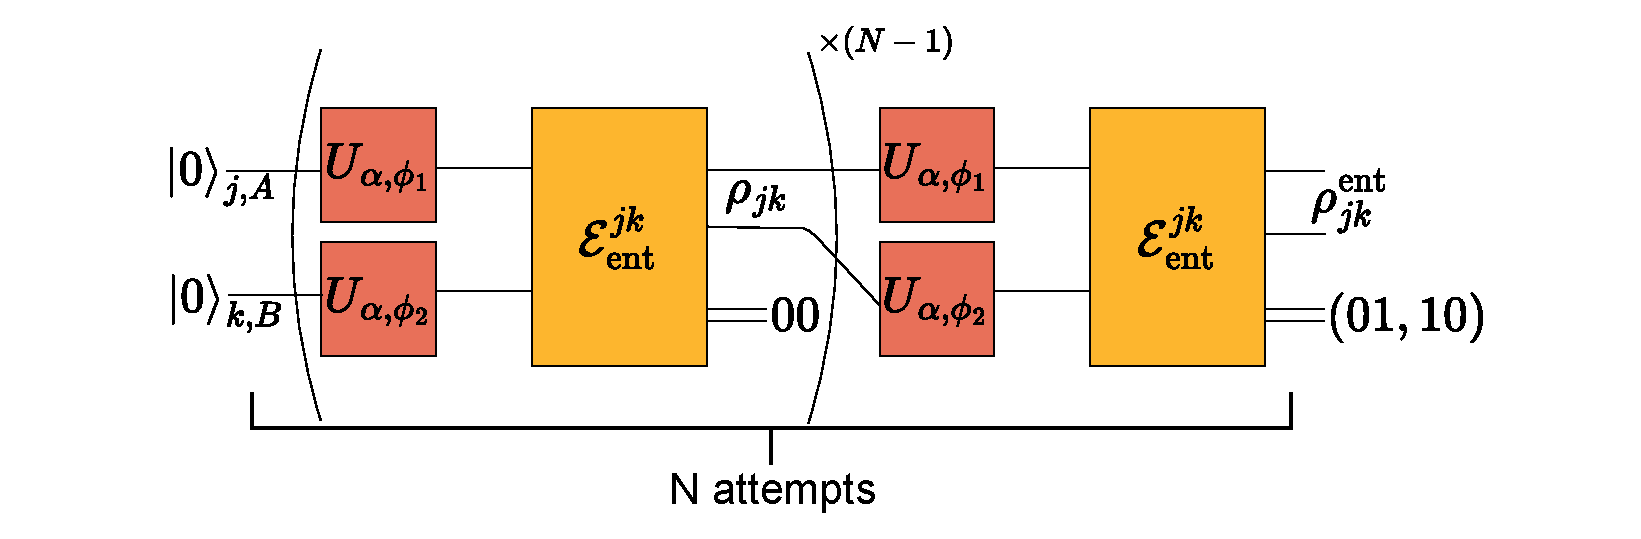
\includegraphics[width=0.8\linewidth]{figs/SI_Fig_5.pdf}
    \caption{\textbf{Stochastic Nature of the Entanglement Protocol.} First ($M$-1) attempts are unsuccessful as $m_{jk}=00$, while $m_{jk}=(01,10)$ at the $M^{\text{th}}$ attempt heralds a successful attempt. An important aspect here that we omit is the swap with nuclear spins $\ket{n}_{j,A}$ and $\ket{n}_{k,B}$, after a successful entanglement is established between electron spin qubits $\ket{0}_{j,A}$ and $\ket{0}_{k,B}$.}
    \label{fig:Si_5}
\end{figure}
The above expression suggests that heralding on zero clicks on both ports leads to a mixed state between qubits $j$ and $k$. Thus, in order to re-utilize it for the next attempt, we propose a controlled laser based spin-initialization depending on if there is a click or not, $U_{\text{init}}$ which performs the following transformation:
\begin{align}
        U_{\text{init}}:\rho_{jk}\to \ket{00}_{j,k}\bra{00}
\end{align}
Now, we repeat this protocol until the measurement outcome is either 01 or 10, as in Figure~\ref{fig:Si_5}. An important aspect here that we omit is the respective swap with nuclear spins $\ket{n}_{j,A}$ and $\ket{n}_{k,B}$, after a successful entanglement is established between electron spin qubits $\ket{0}_{j,A}$ and $\ket{0}_{k,B}$. For our analysis we also assume that the electron-nuclear SWAP gate error is negligible and constant wrt to entanglement error. This assumption allows us to focus largely on entanglement errors arising due to electron spin. This gives the following fidelity and probability of getting clicks only in the $M^{th}$ attempt (assuming $\eta<<1$):
\begin{subequations}
    \begin{align}
        F_{jk} &= \text{cos}^{2}\bigg(\frac{\Delta n_{\phi}}{2}\bigg)\frac{1-\alpha}{1-\alpha\eta}\\
        P_{jk}(M) &= 2\alpha\eta(1-2\alpha\eta)^{N-1}
    \end{align}
\end{subequations} 
Let, $n_{jk}$ be the attempt number which leads to first successful entanglement. As discussed in the main text, this leads to a distribution in $n$:
\begin{equation}
\mathcal{D}_{n} = \{n_{jk}\}_{\substack{1\leq i \leq N_{a} \\ 1 \leq j \leq N_{b}}}
\end{equation}
where each $n_{jk}$ is sampled from the geometric distribution in Eq.(32b), and $N_{a}$ and $N_{b}$ are the number of qubits in system A and B respectively.
\subsection{Thermal Decoherence}
The thermal induced quantum noise acting on the state $\rho$, can be modeled as a generalized amplitude damping channel, $\mathcal{E}_{\text{th}}(\rho)$ given by \cite{Nielsen_Chuang_2010}:
\begin{align}
    &\mathcal{E}_{\text{th}}(\rho) = 
\begin{bmatrix}
(1 - \gamma)\rho_{00} + \gamma p_{\text{th}} & \sqrt{1 - \gamma} \, \rho_{01} \\
\sqrt{1 - \gamma} \, \rho_{01}^* & 1 - (1 - \gamma)\rho_{00} - \gamma p_{\text{th}}
\end{bmatrix}\\
&\text{for a general state }
\rho = 
\begin{bmatrix}
\rho_{00}& \rho_{01} \\
\rho_{01}^* & (1 - \rho_{00})
\end{bmatrix}
\end{align}
where, $\gamma = (1- \text{e}^{-t/T_{1}})$, and $p_{\text{th}}$ is the thermodynamic steady-state probability given by the Boltzmann distribution:
\begin{equation}
    p_{\text{th}} = \frac{\text{e}^{-E_0 / (k_B T)}}{\text{e}^{-E_0 / (k_B T)} + \text{e}^{-E_1 / (k_B T)}} 
= \frac{1}{1 + \text{e}^{-\hbar\omega / (k_B T)}},
\end{equation}
where $E_{1(0)}$ is the energy of the qubit $\ket{1}(\ket{0})$, and $E_1 - E_0 = \hbar\omega$, and $T$ is the local temperature of the qubit environment.
If we start from a state, $\ket{\psi}_{\alpha,\phi} = \sqrt{\alpha}\ket{0} + \text{e}^{i\phi}\sqrt{1-\alpha}\ket{1}$, which corresponds to $\rho_{\alpha,\phi}$:
\begin{align}    \rho_{\alpha,\phi} &= 
    \begin{bmatrix} 
    \alpha & \text{e}^{-i\phi} \, \sqrt{\alpha(1-\alpha)}\\\\
    \text{e}^{i\phi} \, \sqrt{\alpha(1-\alpha)} & 1 - \alpha
    \end{bmatrix} 
\end{align}
Let us look at the expectation value of $\sigma_y$:
\begin{align}
    \langle\sigma_{y}\rangle_{\alpha,\phi} &= 
    2 \, \sqrt{\alpha(1-\alpha)} \, \sin(\phi)
\end{align}
In the presence of a thermal decoherence channel, $\alpha$ is a stochastic variable, hence the averaged state is given by:
\begin{align}
    \overline{\rho}_{\alpha,\phi}(t) &= 
    \begin{bmatrix} 
    \overline{\alpha} & \text{e}^{-i\phi} \, \overline{\sqrt{\alpha(1-\alpha}} \\
    \text{e}^{i\phi} \, \overline{\sqrt{\alpha(1-\alpha)}} & 1 - \overline{\alpha}
    \end{bmatrix}
\end{align}
So we find the following average expectation value of $\sigma_y$:
\begin{align}
    \overline{\langle\sigma_{y}\rangle}_{\alpha,\phi} &= 
    2 \, \overline{\sqrt{\alpha(1-\alpha)}} \, \sin(\phi)
\end{align}


where the overline refers to the average over $\alpha$. Equating Eq.~(40) with Eq.~(34), we find the following:
\begin{subequations}
\begin{align}
    \overline{\sqrt{\alpha(1-\alpha)}} &\approx \sqrt{1-\gamma}\sqrt{\alpha(1-\alpha)} = \text{e}^{-\frac{t}{2T_{1}}}\sqrt{\alpha(1-\alpha)}\\
    \overline{\alpha} &= \text{e}^{-\frac{t}{T_{1}}}\alpha + (1- \text{e}^{-\frac{t}{T_{1}}})p_{\text{th}}
\end{align}    
\end{subequations}
Thus, we get following expression for thermal-induced decoherence:
\begin{equation}
\overline{\langle\sigma_{y}\rangle}_{\alpha,\phi} = 2\text{e}^{-\frac{t}{2T_{1}}}~\sqrt{\alpha(1-\alpha)}~\text{sin}(\phi) 
\end{equation}

\subsection{Dephasing Channel}
Let $\mathcal{E}_{\text{dep}}(\rho)$ be a pure dephasing channel given by \cite{Nielsen_Chuang_2010}:
\begin{equation}
    \mathcal{E}_{\text{dep}}:\rho\to (1-p_{\text{dep}})\rho + p_{\text{dep}}\sigma_{\text{z}}\rho\sigma_{\text{z}}
\end{equation}
% Further we define coherence of a system as $M_{coh}$:
% \begin{equation}
%     M_{coh}(\rho;
%     \tau;n_{\phi}) = |\dashbar{\langle\sigma_{y}\rangle}_{\rho}|
% \end{equation}
% \begin{figure}
%     \centering
%     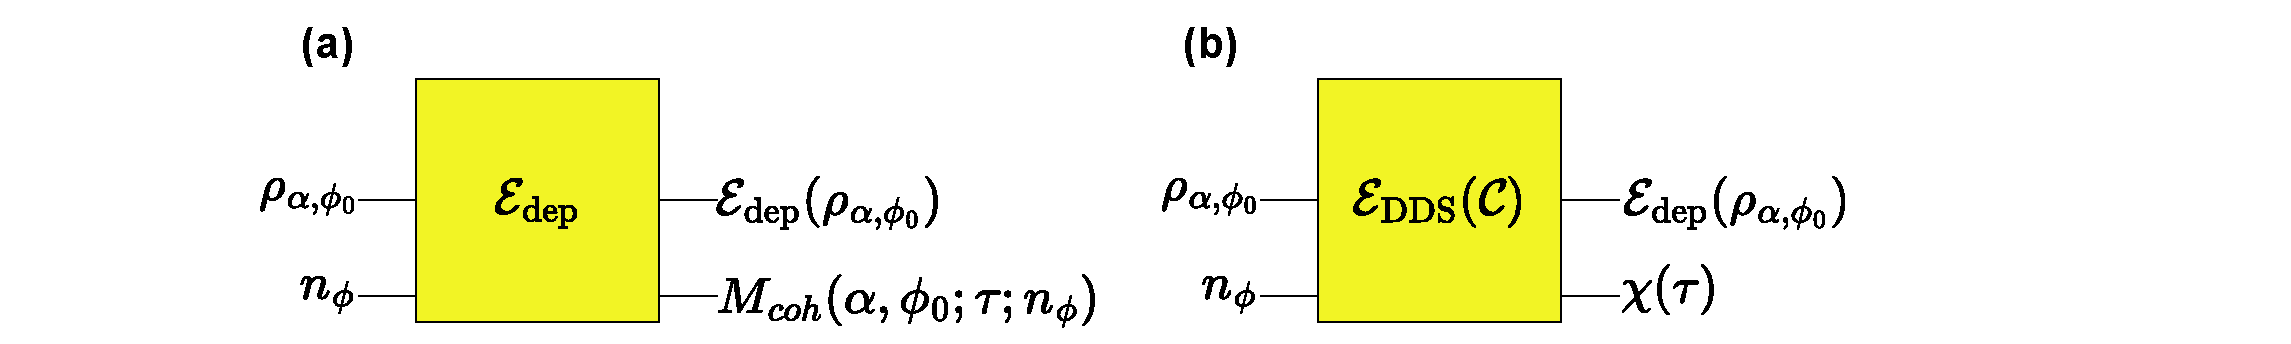
\includegraphics[width=\linewidth]{figs/SI_Fig_6.pdf}
%     \caption{\textbf{(a)} Dephasing Channel $\mathcal{E}_{\text{dep}}$ depends on the noise spectrum $n_{\phi}$, and outputs a coherence function $M_{coh}\equiv |\dashbar{\langle\sigma_{y}\rangle}|$. \textbf{(b)} Dynamical Decoupling Channel $\mathcal{E}_{\text{DDS}}$ modeled as dephasing channel which outputs $M_{coh}\equiv \text{e}^{-\chi(\tau)}=\text{e}^{-(\tau/T_{2})^{n}}$}
%     \label{fig:enter-label}
% \end{figure}
% where the angled bracket corresponds to expectation value for the quantum evolution of $\rho$ (accounts for the pure dephasing), and tilde corresponds to ensemble average (accounts for inhomogenous broadening based dephasing), which averages on the stochastic phase noise $n_{\phi}$ of the control or environment from one experimental run to another, and $\tau$ is the experimental duration of dephasing. Similar to the previous case, we start from a state, $\ket{\psi}_{\alpha,\phi} = \sqrt{\alpha}\ket{0} + \text{e}^{i\phi}\sqrt{1-\alpha}\ket{1}$.
Similar to the previous case, we start from a state, $\ket{\psi}_{\alpha,\phi} = \sqrt{\alpha}\ket{0} + \text{e}^{i\phi}\sqrt{1-\alpha}\ket{1}$. In the presence of dephasing channel, $\phi$ is a stochastic variable, hence the ensemble average state is given by:
\begin{align}
    \dashbar{\rho_{\alpha,\phi}} &= \begin{bmatrix} 
    \alpha & \dashbar{\text{e}^{-i\phi}}\sqrt{\alpha(1-\alpha)} \\\\
    \dashbar{\text{e}^{i\phi}}\sqrt{\alpha(1-\alpha)} & 1 -\alpha
\end{bmatrix}
\end{align}
This gives the following ensemble average expectation value of $\sigma_y$:
\begin{align}
\dashbar{\langle\sigma_{y}\rangle}_{\alpha,\phi} &= 2\sqrt{\alpha(1-\alpha)}~\dashbar{\text{sin}(\phi)}
\end{align}

Here the angled bracket corresponds to the expectation value for the quantum evolution of $\rho$ (accounts for the pure dephasing), and tilde corresponds to the ensemble averaging (accounts for inhomogeneous broadening based dephasing), which averages on the stochastic phase noise $n_{\phi}$ of the control or environment from one experimental run to another. 

Suppose, $\phi$ is centered around $\phi_{0}$ such that, $\phi=\phi_{0} + n_{\phi}$, where $n_{\phi}$ is the stochastic phase variable.
\begin{equation}
     |\dashbar{\langle\sigma_{y}\rangle}_{\alpha,\phi_{0}}| = 2\sqrt{\alpha(1-\alpha)}\text{sin}(\phi_{0})|~\dashbar{\text{cos}(n_{\phi})}| + \text{cos}(\phi_{0})~|\dashbar{\text{sin}(n_{\phi})}|
\end{equation}
For a system characterized for the initial state  $\ket{Y_{+}}=\frac{\ket{0}+i\ket{1}}{\sqrt{2}}$ \cite{Biercuk_2011}:
\begin{equation}
    |\dashbar{\langle\sigma_{y}\rangle}| = |\dashbar{\text{cos}(n_{\phi})}| = \text{e}^{-\chi_{\text{dep}}(\tau)}
\end{equation}
Here the decoherence function $\chi_{\text{dep}}(\tau)$ is given by:
\begin{equation}
    \chi_{\text{dep}}(\tau) = \bigg(\frac{\tau}{T_{\phi}}\bigg)^{z_{\phi}} + \bigg(\frac{\tau}{T_{\text{inh}}}\bigg)^{z_{\text{inh}}}
\end{equation}
Here $\tau$ is the experimental duration of dephasing, $1/T_{\phi}$ is the pure-dephasing rate and $1/T_{\text{inh}}$ is the inhomogeneous-broadening rate. Further, depending on the noise spectra of these individual sources, we assume a scaling factor of $z_{\phi}$ and $z_{\text{inh}}$ respectively.

\subsection{Composing Thermal Decoherence with a Dephasing Channel}
In the presence of thermal decoherence and dephasing, both $\alpha$ and $\phi$ are stochastic variables, which means the coherence function needs to be averaged over both, yielding the following:
\begin{equation}    \dashbar{\overline{\rho_{\alpha,\phi}}} = 
    \begin{bmatrix} 
    \overline{\alpha} & \dashbar{\text{e}^{-i\phi}} \, \overline{\sqrt{\alpha(1-\alpha)}} \\\\
    \dashbar{\text{e}^{i\phi}} \, \overline{\sqrt{\alpha(1-\alpha)}} & 1 - \overline{\alpha}
    \end{bmatrix}
\end{equation}
\begin{subequations}
    \begin{align}
     \dashbar{\overline{\langle\sigma_{y}\rangle}}_{\alpha,\phi} &= 
    2 \, \overline{\sqrt{\alpha(1-\alpha)}} \, \dashbar{\sin(\phi)}\\
    &= 2~\sqrt{\alpha(1-\alpha)}~\text{e}^{-(\frac{\tau}{2T_{1}}+\chi_{\text{dep}}(\tau))}\\
    &= 2~\sqrt{\alpha(1-\alpha)}~\text{e}^{-\chi^{*}(\tau)}
    \end{align}
\end{subequations}
where we introduced the effective decoherence function $\chi^{*}(\tau)$:
\begin{subequations}
\begin{align}
   \chi^{*}(\tau) &= \frac{\tau}{2T_{1}}+\chi_{\text{dep}}(\tau)\\
   &= \frac{\tau}{2T_{1}}+\bigg(\frac{\tau}{T_{\phi}}\bigg)^{z_{\phi}} + \bigg(\frac{\tau}{T_{\text{inh}}}\bigg)^{z_{\text{inh}}} \simeq \bigg(\frac{\tau}{T^{*}_{2}}\bigg)^{z^{*}}
\end{align}    
\end{subequations}
The scaling $z^{*}$ is the effective asymptotic scaling factor depending on $\tau$ and individual scalings $z_{\phi}$ and $z_{\text{inh}}$. In the main text we characterize a dynamical decoupling sequence for initial state along the bloch-axis y (i.e. $\alpha=1/2, \phi= \pi/2$), which gives:
\begin{equation}
    \chi_{\text{dds}}(\tau) = \bigg(\frac{\tau}{T_{2}}\bigg)^{z_{\text{dds}}}
\end{equation}
Since the dynamical decoupling sequence mainly reduces the inhomogeneous phase noise, we assume that $T_{\text{inh}}$ increases to $\kappa_{\text{dds}}T_{\text{inh}}$, where $\kappa_{\text{dds}}>1$ is a factor of improvement. From Eq. (51b) and Eq.(52), we get the following:
\begin{subequations}
    \begin{align}
      \bigg(\frac{\tau}{T_{2}}\bigg)^{z_{\text{dds}}} &= \frac{\tau}{2T_{1}}+\bigg(\frac{\tau}{T_{\phi}}\bigg)^{z_{\phi}} + \bigg(\frac{\tau}{\kappa_{\text{dds}}T_{\text{inh}}}\bigg)^{z_{\text{inh}}}\\
      &= \frac{\tau}{2T_{1}} + \chi^{\prime}_{\text{dep}}(\tau)
    \end{align}
\end{subequations}
Assuming $T_{1}>>T_{2}$ this becomes:
\begin{equation}
     \bigg(\frac{\tau}{T_{2}}\bigg)^{z_{\text{dds}}} \approx \chi^{\prime}_{\text{dep}}(\tau)
\end{equation}
Thus, in the presence of thermal decoherence, phase noise and a dynamical decoupling sequence, $\chi^{\prime}_{\text{dep}}(\tau)$ quantifies the effective decoherence rate of the phase.
\subsection{Combining the Entanglement Protocol and Dynamical Decoupling Sequence}
The operation order for a single entanglement attempt after performing dynamical decoupling is shown in Fig. \ref{fig:singleentanglementblock}.
\begin{figure}
    \centering
    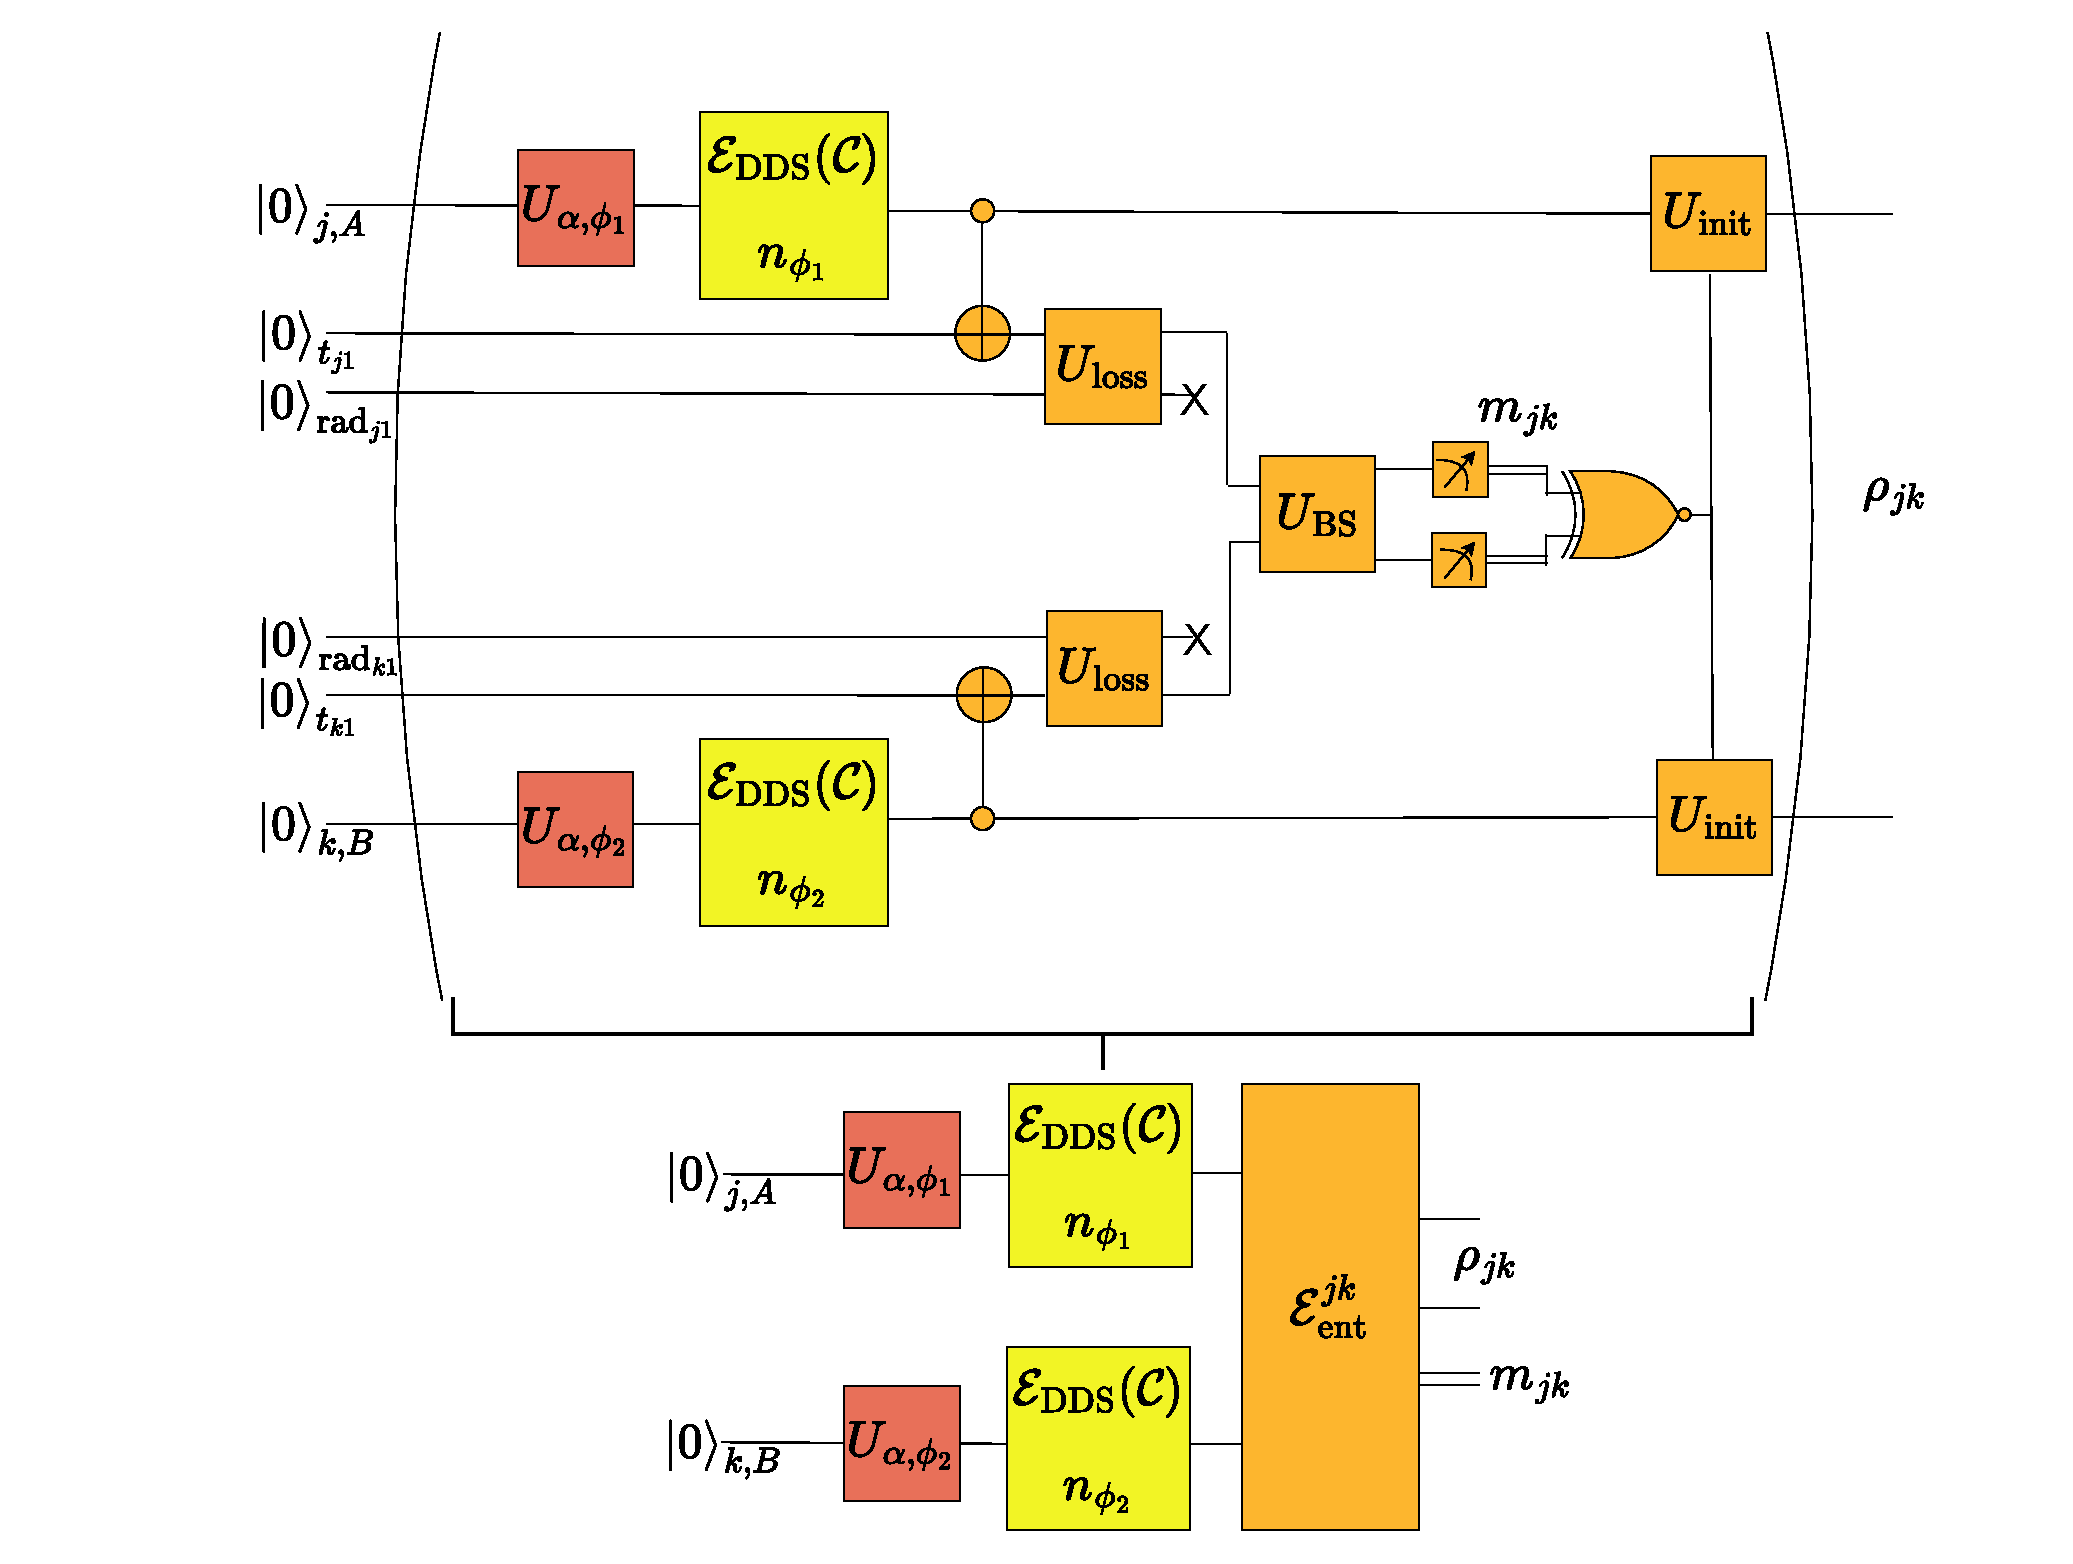
\includegraphics[width=0.9\linewidth]{figs/SI_Fig_7.pdf}
    \caption{A single attempt of combination of Dynamical Decoupling Channel and Single Photon Entanglement for a qubit pair $(j_{A},k_{B})$}
    \label{fig:singleentanglementblock}
\end{figure}
In Eq.40, we estimate the entanglement fidelity $F_{exp}$ for a single run, but in order to make it closer to experiments, one has to take an ensemble average for both thermal and dephasing channels:
\begin{equation}
    \dashbar{\overline{F}}_{exp} = \overline{\bigg(\frac{1-\alpha}{1-\alpha\eta}\bigg)}\dashbar{\bigg(\text{cos}^2\bigg(\frac{\Delta n_{\phi}}{2}  \bigg)\bigg)}
\end{equation}
Assuming that $\eta<<1$, we get the following:
\begin{equation}
   \dashbar{\overline{F}}_{\text{exp}}= (1-\overline{\alpha})\bigg(\frac{1 + \dashbar{\text{cos}(\Delta n_{\phi})}}{2}\bigg)
\end{equation}
Let us break down the ensemble averaging:
    \begin{align}
        \dashbar{\text{cos}(\Delta n_{\phi})} = \dashbar{\text{cos}(n_{\phi_{1}} - n_{\phi_{2}})} = \dashbar{\text{cos}(n_{\phi_{1}})}~\dashbar{\text{cos}(n_{\phi_{2}})} + \dashbar{\text{sin}(n_{\phi_{1}})}~\dashbar{\text{sin}(n_{\phi_{2}})}
    \end{align}
Since $n_{\phi_{1}}$ and $n_{\phi_{2}}$ correspond to noise spectra on two spatially separated identical systems, we assume them to be identical and independent. The dynamical decoupling sequence improves the phase coherence for the entanglement protocol $(T_2^*\rightarrow T_2)$, therefore:
\begin{subequations}
    \begin{align}
        |\dashbar{\text{cos}(n_{\phi_{1}})}| &= \text{e}^{-\chi^{\prime}_{1,\text{dep}}(\tau)}\\
        |\dashbar{\text{cos}(n_{\phi_{2}})}| &= \text{e}^{-\chi^{\prime}_{2,\text{dep}}(\tau)}
    \end{align}
\end{subequations}
Here, $\chi^{\prime}_{1(2),\text{dep}}$ is given by Eq.(54).
Without loss of generality, let's assume the following convention:
\begin{subequations}
    \begin{align}
        &\dashbar{\text{cos}(n_{\phi_{1}})} = p; ~\dashbar{\text{sin}(n_{\phi_{1}})} = q\\
        &\dashbar{\text{cos}(n_{\phi_{2}})} = r; ~\dashbar{\text{sin}(n_{\phi_{2}})} = s\\
        &P = |\dashbar{\text{cos}(\Delta n_{\phi_{}})}| = |pr + qs|
    \end{align}
\end{subequations}
By triangle inequality of distance measures, we have the following:
\begin{equation}
   |p||r| - |q||s|  \le P \le |p||r| + |q||s| 
\end{equation}
We further have the following inequalities:
\begin{subequations}
\begin{align}
    &\dashbar{\text{cos}^{2}(n_{\phi_{1}})} = 1 - \dashbar{\text{sin}^{2}(n_{\phi_{1}})} \ge \dashbar{\text{cos}(n_{\phi_{1}})}~^{2} = p^{2}\\
    &\implies 1 - p^2 \ge \dashbar{\text{sin}^{2}(n_{\phi_{1}})} \ge \dashbar{\text{sin}(n_{\phi_{1}})}~^{2} = q^{2} \\
    &\implies |q| \le \sqrt{1-p^2} 
\end{align}
\end{subequations}
Similarly, we have: $|s| \le \sqrt{1-r^2}$.

From this we get:
\begin{equation}
    P \ge |p||r| - |q||s| \ge |p||r| - \sqrt{1-p^2}\sqrt{1-q^2}
\end{equation}
Since $|p|=\text{e}^{-\chi^{\prime}_{1,\text{dep}}(\tau)}$ and $|r|=\text{e}^{-\chi^{\prime}_{2,\text{dep}}(\tau)}$, we get:
\begin{equation}
    \dashbar{\text{cos}(\Delta n_{\phi})} \ge \text{e}^{-(\chi^{\prime}_{1,\text{dep}}(\tau)+\chi^{\prime}_{2,\text{dep}}(\tau))} - \sqrt{1 - \text{e}^{-2\chi^{\prime}_{1,\text{dep}}(\tau)}}\sqrt{1 - \text{e}^{-2\chi^{\prime}_{2,\text{dep}}(\tau)}}
\end{equation}
Thus, by combining Eq.~(41b), (56) and (63), we get the following:
\begin{tcolorbox}[breakable, colback=white]
\begin{align}
\dashbar{\overline{F_{\text{exp}}(\tau)}} 
&\ge \bigg(1 - e^{-\frac{\tau}{T_1}} \alpha - (1 - e^{-\frac{\tau}{T_1}}) p_{\text{th}} \bigg) \nonumber \\
&\quad \times \bigg( \frac{1 + e^{-(\chi'_{1,\text{dep}}(\tau) + \chi'_{2,\text{dep}}(\tau))} 
- \sqrt{1 - e^{-2\chi'_{1,\text{dep}}(\tau)}} \sqrt{1 - e^{-2\chi'_{2,\text{dep}}(\tau)}}}{2} \bigg)
\end{align}
\end{tcolorbox}

Here, we assumed that the $T_{1}$ process and $T_{1}$ timescale for both systems are identical. In order to estimate the error of this protocol $\epsilon$, we use the following definition of distance measure $\mathcal{D}$ between two states $\rho$ and $\sigma$:
\begin{equation}
    \mathcal{D}(\rho,\sigma) = \frac{1}{2}\text{Tr}|\rho-\sigma|
\end{equation}
We use the following property:
\begin{subequations}
\begin{align}
    &1 - F(\rho,\sigma) \le \mathcal{D}(\rho,\sigma) \le \sqrt{1 - F(\rho,\sigma)^2}\\
    &1 - \overline{F(\rho,\sigma)} \le \overline{\mathcal{D}(\rho,\sigma)} \le \sqrt{1 - \overline{F(\rho,\sigma)
    }^2}~: \text{By Jensen's Inequality}
\end{align}
\end{subequations}
This gives:
\begin{equation}
    \dashbar{\overline{\mathcal{D}_{jk}(\tau)}}_{\text{min}} = 1 - \dashbar{\overline{{F}_{exp}(\tau)}}
\end{equation}
Using the universality principle that an arbitrary 2-qubit gate can implemented by a 1-qubit unitary and a CNOT gate, we get the following expression for the average 2-qubit error between qubits $j$ and $k$:
\begin{equation}
    \epsilon_{jk}(\tau) = \text{max}(\dashbar{\overline{\mathcal{D}_{jk}(\tau)}}_{\text{min}} + \epsilon_{\text{1-qubit}})
\end{equation}
Including the $N$-pulse CPMG unitary errors modifies the above error as follows:
\begin{equation}
   \epsilon_{jk}(\tau,N) = \text{max}(\dashbar{\overline{\mathcal{D}_{jk}(\tau)}}_{\text{min}}) + (2N+1)\epsilon_{1-\text{qubit}} 
\end{equation}
% \begin{equation}
%  \boxed{
%  \quad
%  \epsilon_{jk}(\tau) = \sqrt{1 - \bigg(\frac{1-\alpha}{1-\alpha\eta}\bigg(\frac{1 +\text{e}^{-(\chi_{1}(\tau)+\chi_{2}(\tau))} - \sqrt{1 - \text{e}^{-2\chi_{1}(\tau)}}\sqrt{1 - \text{e}^{-2\chi_{2}(\tau)}}}{2}\bigg)\bigg)^{2} }
%  \quad
%  } 
% \end{equation}

Combining Eq. Eq.~(64), (67) and (69) gives us our final expression for the average 2-qubit error between qubits $j$ and $k$:

\begin{tcolorbox}[breakable, colback=white]
\begin{align}
&\epsilon_{jk}(\tau,N, T_{1}, T_{2j}, T_{2k}, z_{j,\text{dds}}, z_{k,\text{dds}} ) \nonumber\\&=
 1 - \left(1 - \text{e}^{-\frac{\tau}{T_{1}}}\alpha 
- (1 - \text{e}^{-\frac{\tau}{T_{1}}})\,p_{\text{th}}\right) \notag \\
&\quad \left. \times 
\left(
\frac{1 +\text{e}^{-(\chi^{\prime}_{j,\text{dep}}(\tau)+\chi^{\prime}_{k,\text{dep}}(\tau))} 
- \sqrt{1 - \text{e}^{-2\chi^{\prime}_{j,\text{dep}}(\tau)}}
\sqrt{1 - \text{e}^{-2\chi^{\prime}_{k,\text{dep}}(\tau)}}}{2}
\right) \right. \notag \\
&\quad  + (2N+1)\epsilon_{1\text{-qubit}} 
\end{align}
\end{tcolorbox}

The $M$-attempts composition of the global decoupling channel with pairwise entanglement blocks is summarized in Fig. \ref{fig:globaldecouplingchannel}.

\begin{figure}
    \centering
    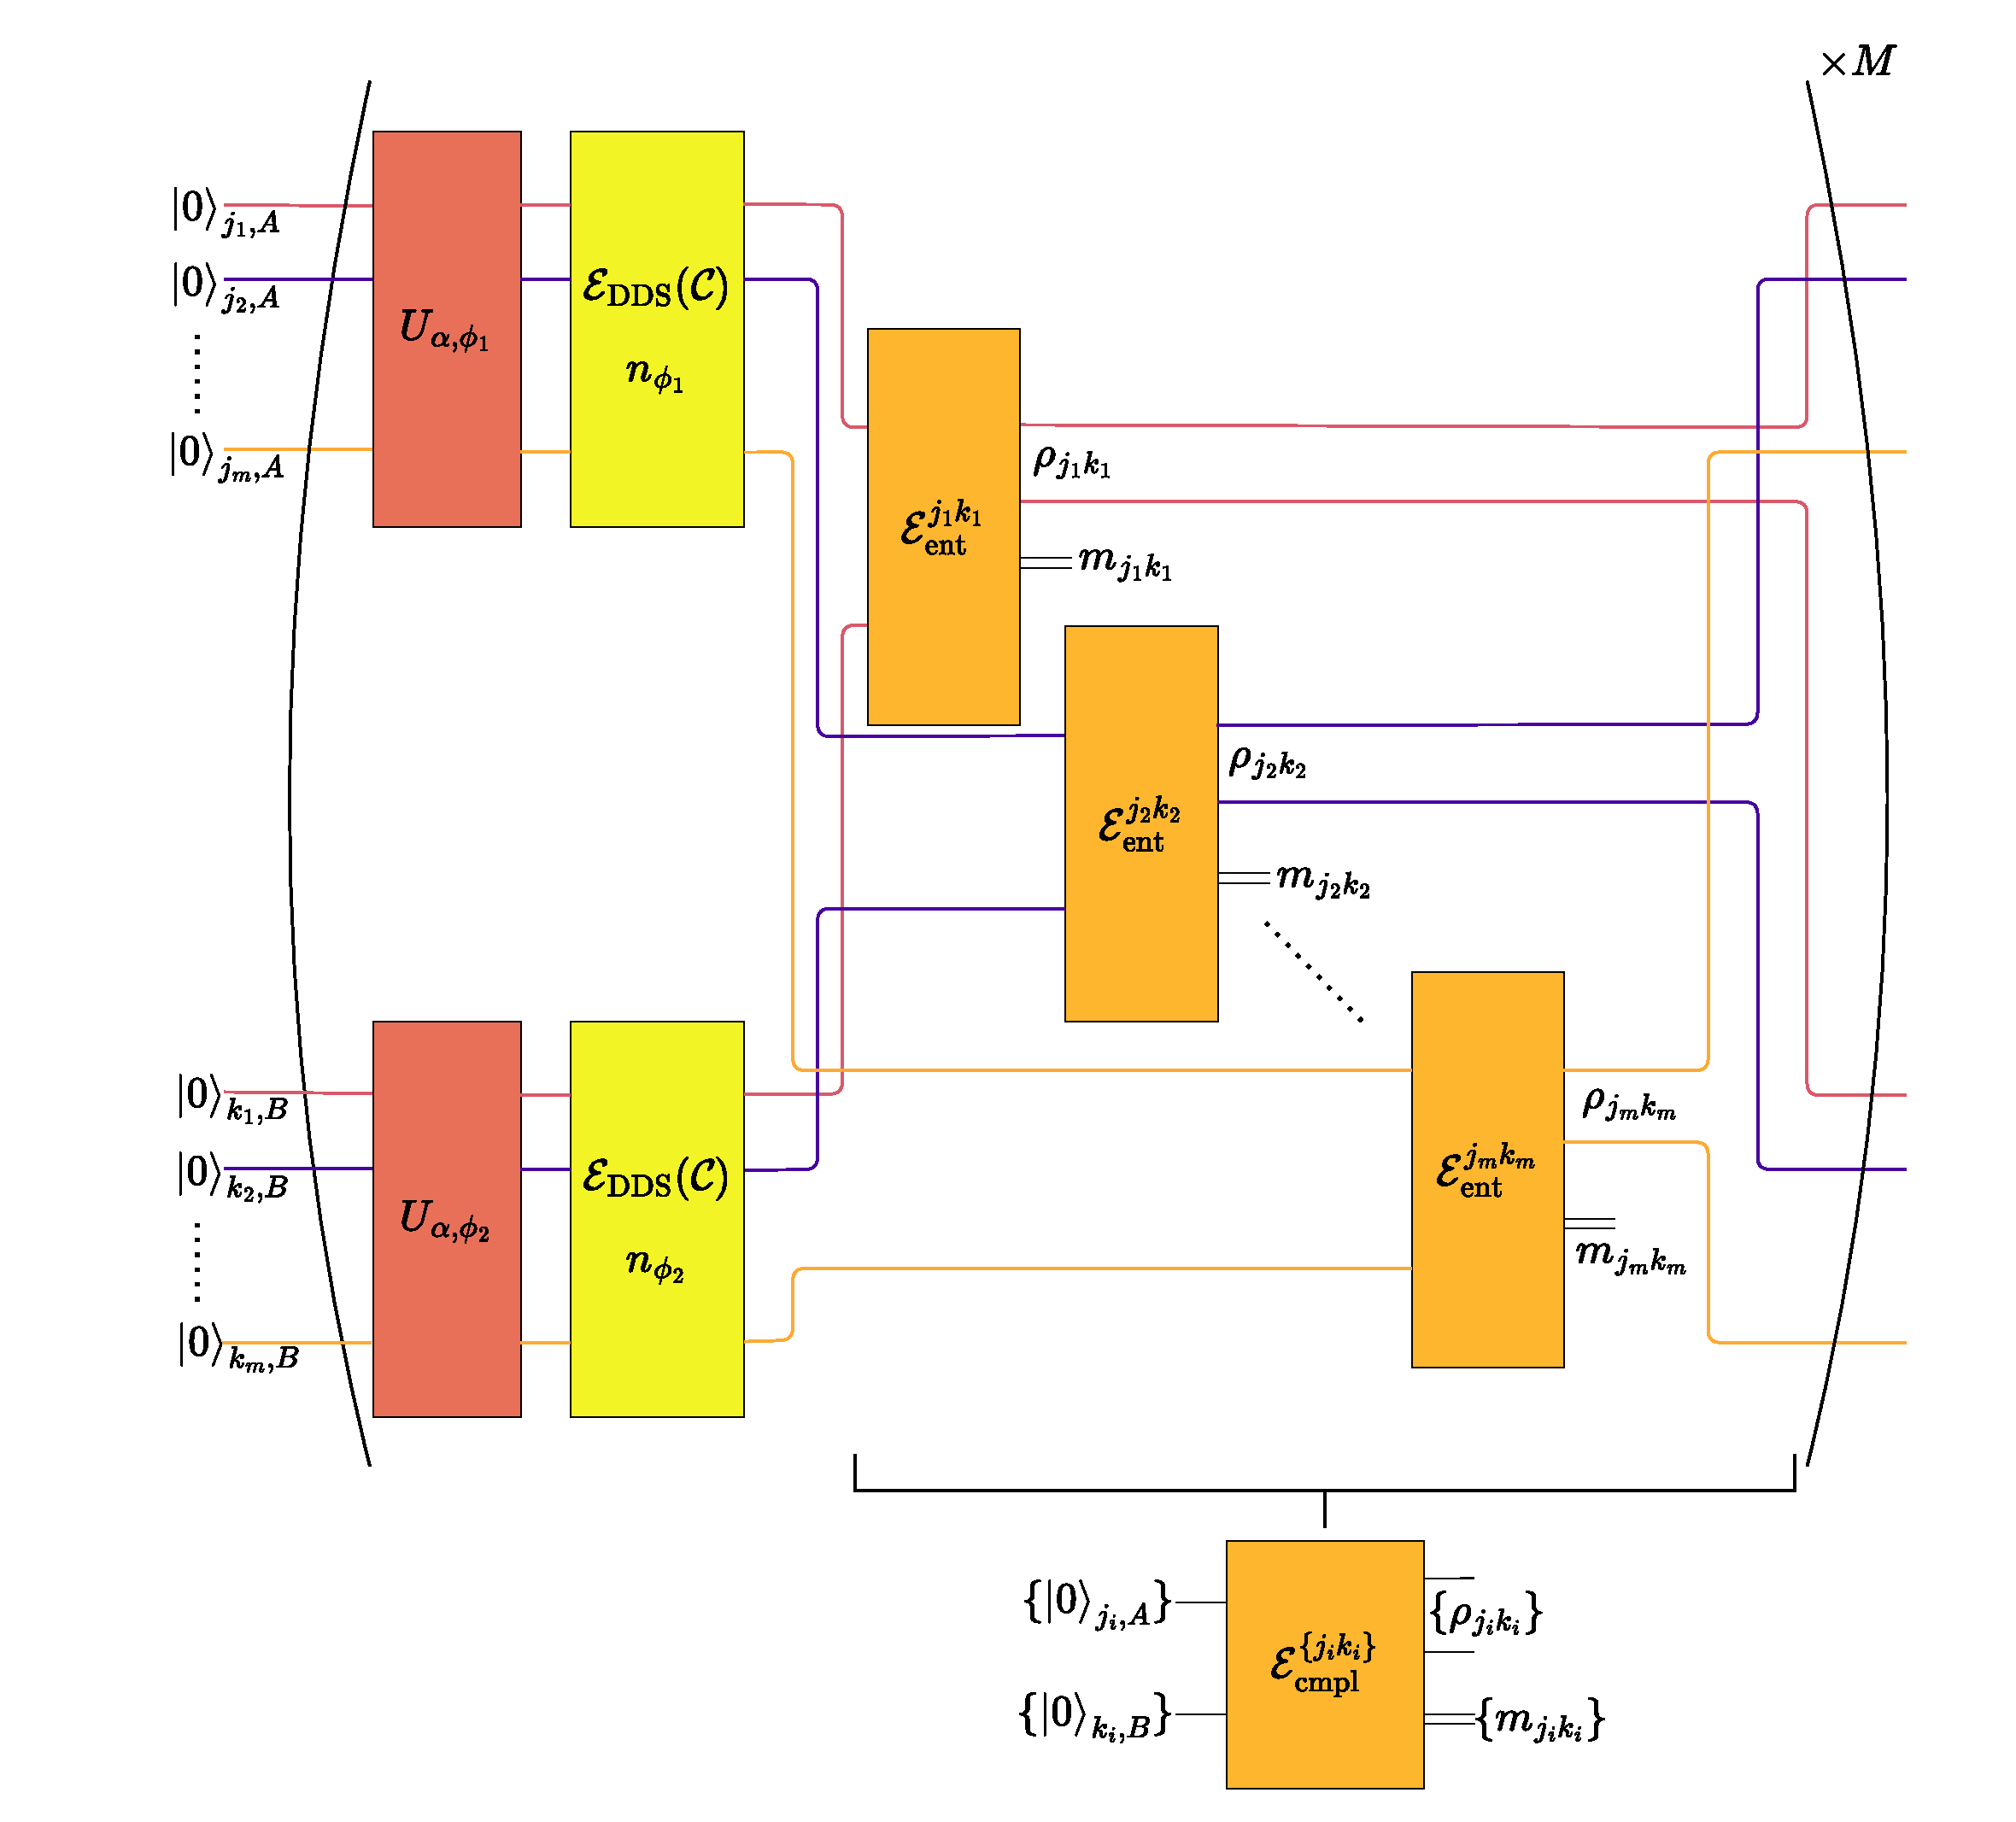
\includegraphics[width=0.9
    \linewidth]{figs/SI_Fig_8.pdf}
    \caption{$M$ attempts of composing the global decoupling channel $\mathcal{E}_{\text{DDS}}$ and pairwise entanglement blocks $\{\mathcal{E}^{j_{i}k_{i}}_{\text{ent}} \}$ given by the compilation strategy.}
    \label{fig:globaldecouplingchannel}
\end{figure}

For completeness, the full end-to-end protocol, executed repeatedly over $M$ attempts, is shown in the block diagram of Fig. \ref{fig:fullblockdiagram}.

\begin{figure}
    \centering
    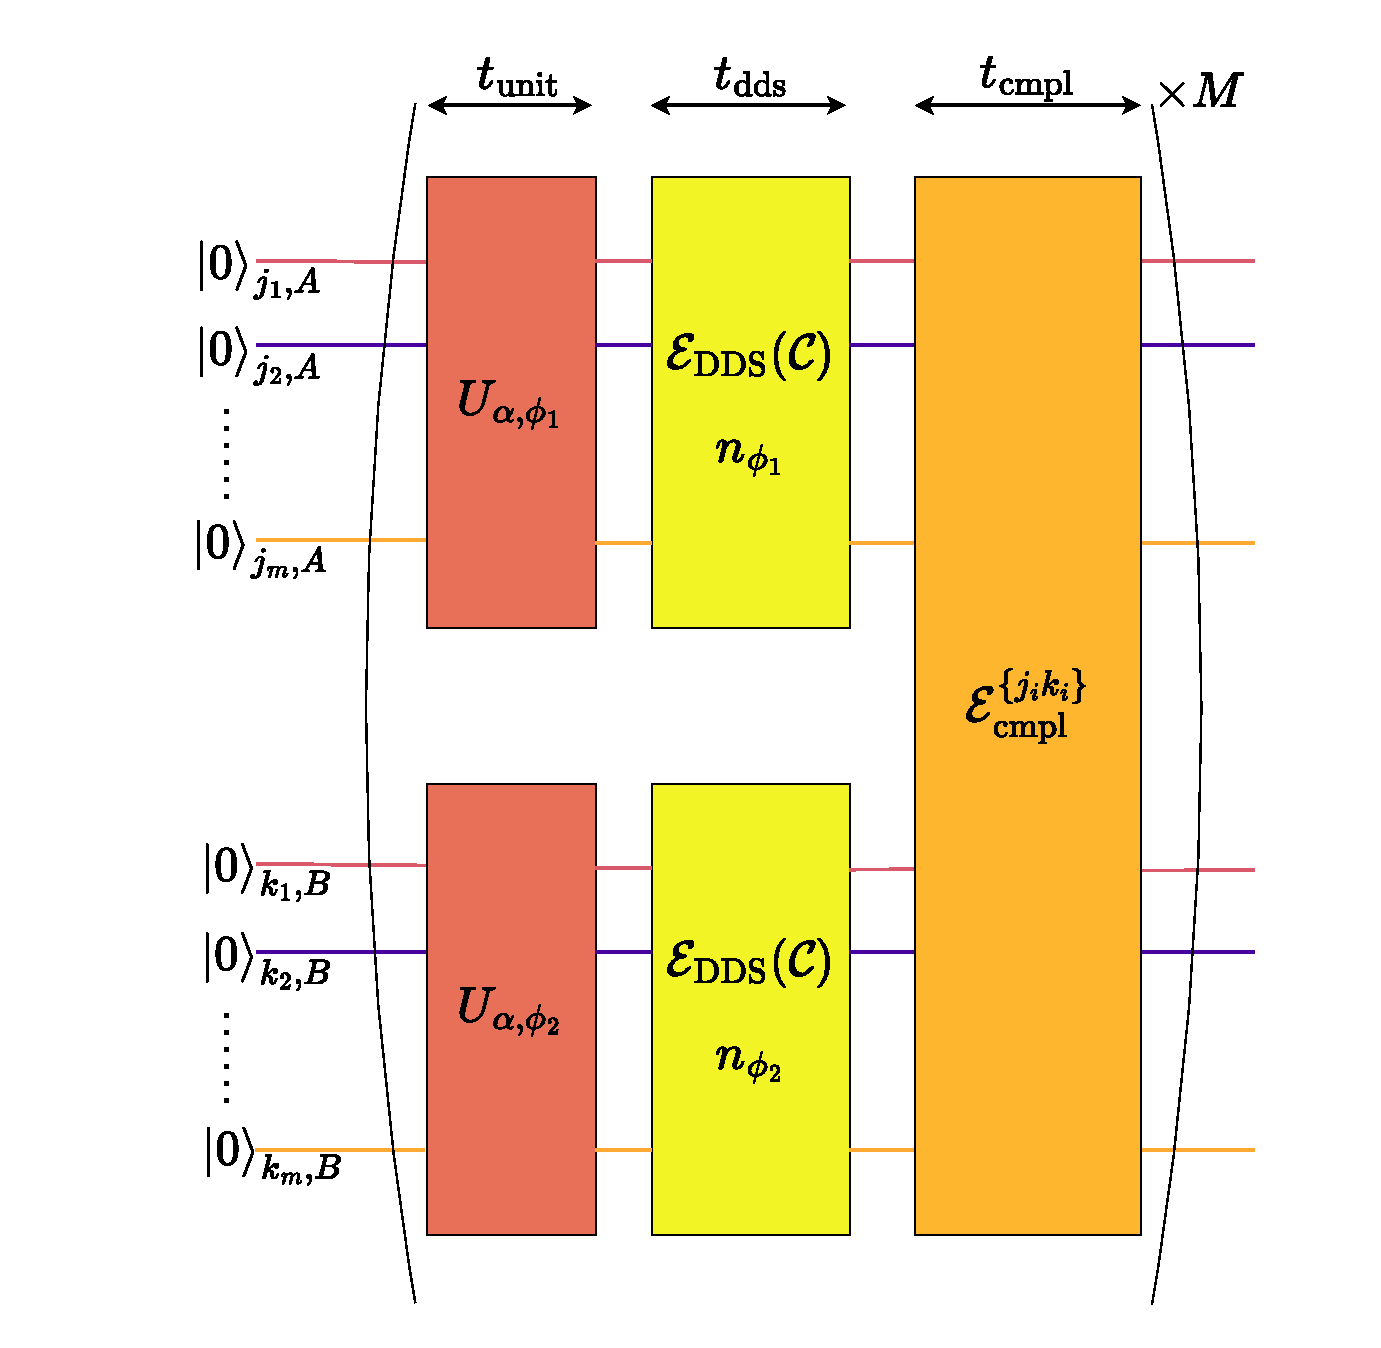
\includegraphics[width=0.6\linewidth]{figs/QCT.pdf}
    \caption{Block diagram of the full protocol repeated $M$ times.}
    \label{fig:fullblockdiagram}
\end{figure}

\subsection{Thermal Budget}
\subsubsection{Cold-Plate Stage}
The $T_{1}$ and $T_{2}$ parameters in the previous section also depend on the local temperature of the SiV$^-$ qubit. This section discusses about modeling the thermal budget of the system.
We assume a train of N pulses, each containing an energy of $E_{\text{pulse}}$, having pulse length $t_{\text{pul}}$, and inter-pulse duration $t_{\text{ip}}$. This gives measurement time $t_{\text{dds}} = \text{N}(t_{\text{pul}} + t_{\text{ip}})$. Suppose the heat-capacity of the system is $C_{\text{sys}}$, the maximum cooling power available in the cryostat is $P_{\text{cool}}$ and the heat-load at the qubit stage is $P_{\text{stage}}$. We assume that the qubit is at the cold-plate stage of the dilution refrigerator.
% We get the following approximate relation for temperature of the system at the end of the full pulse train:
% \begin{subequations}
% \begin{align}
%   T_{\mathrm{sys}}
%   &= T_{\mathrm{cryo}}, 
%   &\text{if}\quad \frac{E_{\mathrm{pulse}}}{t_{\mathrm{ip}}} \le P_{\mathrm{cool}},\\
%   T_{\mathrm{sys}}
%   &= T_{\mathrm{cryo}} + \bigg(\frac{E_{\mathrm{pulse}}}{t_{\text{ip}}}-P_{\text{cool}}\bigg)\frac{t_{\text{dds}}}{C_{\text{sys}}},
%   &\text{if}\quad \frac{E_{\mathrm{pulse}}}{t_{\mathrm{ip}}} > P_{\mathrm{cool}}.
% \end{align}
% \end{subequations}

\begin{figure}
    \centering
    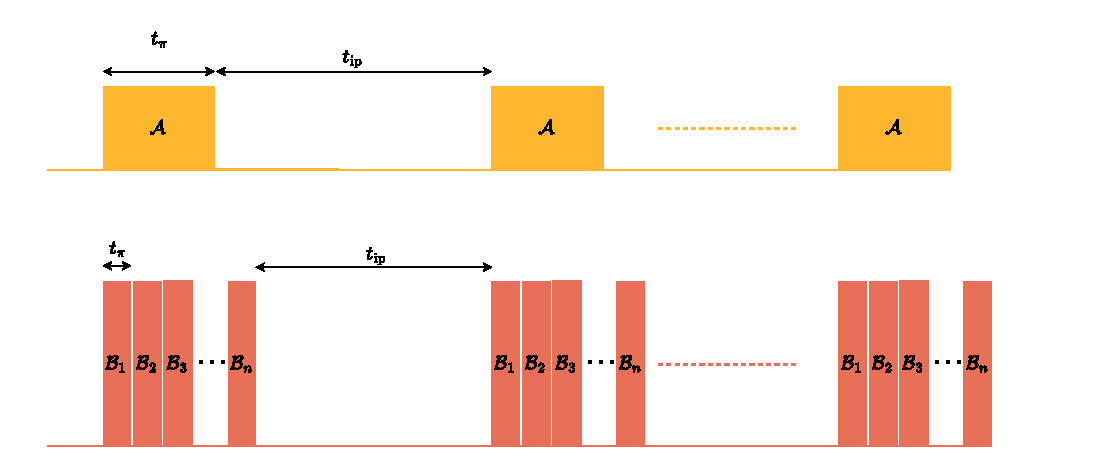
\includegraphics[width=0.9\linewidth]{figs/pulses.pdf}
    \caption{Pulse level diagram}
    \label{fig:enter-label}
\end{figure}


Since the qubit interacts via strain coupling, the approximate energy-density contained per unit mechanical pulse is given by:
\begin{equation}
    u_{\text{mech}}  = \frac{1}{2}\mathrm{Y}_{\text{dia}}\epsilon_{\text{str}}^{2}
\end{equation}
Here, $\mathrm{Y}_{\text{dia}}$ is the Young's modulus of diamond, $\epsilon
_{\text{str}}$ is the strain amplitude for the mechanical wave. With $c_{\text{dia}}$ the speed of sound in diamond, the intensity of the propagating pulse is given by:
\begin{equation}
    \text{I}_{\text{mech}} =  u_{\text{mech}} c_{\text{dia}}  = \frac{1}{2}\mathrm{Y}_{\text{dia}}\epsilon_{\text{str}}^{2}c_{\text{dia}}
\end{equation}
Further, suppose the wave is confined within an aperture area given by $\sim\lambda_{\text{mech}}^{2}$, where $\lambda_{\text{mech}}$ is the wavelength of the mechanical wave. Then the power contained in the pulse is given by:
\begin{equation}
    P_{\text{mech}} = \frac{1}{2}\mathrm{Y}_{\text{dia}}\epsilon_{\text{str}}^{2}c_{\text{dia}}\lambda_{\text{mech}}^{2}
\end{equation}
Given the transduction efficiency $\eta_{\text{tr}}$ from microwave mode to mechanical mode, the microwave power delivered to the sample near the cold-plate stage is given by:
\begin{equation}
    P_{\text{MW}} = \frac{1}{2\eta_{\text{tr}}}\mathrm{Y}_{\text{dia}}\epsilon_{\text{str}}^{2}c_{\text{dia}}\lambda_{\text{mech}}^{2} \propto \epsilon_{\text{str}}^{2}
\end{equation}
We plug in typical values from the literature: $\eta_{\text{tr}}=0.35$ \cite{mirhosseini2020superconducting}, $\mathrm{Y}_{\text{dia}}\sim1000$ GPa \cite{brisDiamondProperties}, $c_{\text{dia}}\sim 12000$ m/s \cite{brisDiamondProperties}, $\lambda_{\text{mech}}\sim 2.4~\mu$m (for 5 GHz). This gives the following:
\begin{equation}
    P_{\text{MW}} \approx 9.87\times10^{4}\epsilon_{\text{str}}^{2} \text{W}
\end{equation}

\begin{figure}
    \centering
    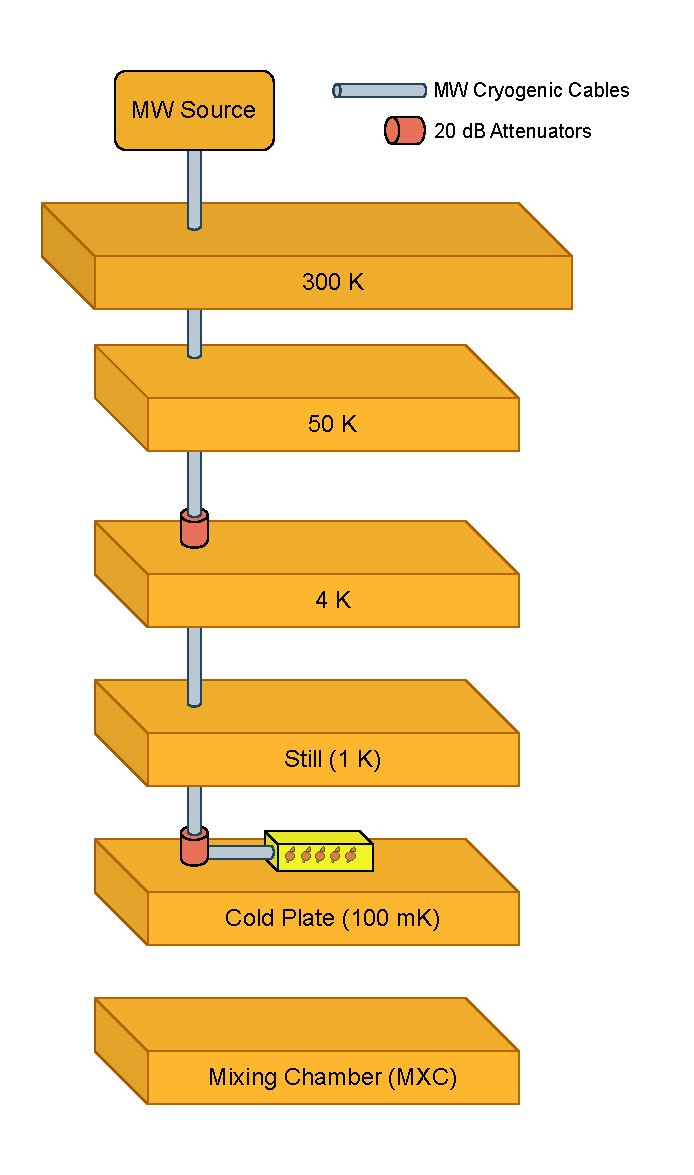
\includegraphics[width=0.5\linewidth]{figs/thermal_model.pdf}
    \caption{Dilution Fridge Configuration \cite{krinner2019engineering}}
    \label{fig:dil_fridge}
\end{figure}
For $\epsilon_{\text{str}}= 1.56\times 10^{-6}$ (See SI Sec. \ref{sec:straindriving}), we get $P_{\text{MW}}\approx0.24~\mu$W. We assume the stages of dilution fridge as in Figure \ref{fig:dil_fridge} (adapted from \cite{krinner2019engineering}), which has the following stages: Room temperature 300 K - 50 K - 4 K - 1 K - 100 mK (Cold Plate, CP) - MXC (Mixing Chamber) with 20 dB attenuators at 4 K, 100 mK, and MXC. The major sources of heat dissipation at the CP stage are:
\begin{itemize}
    \item Active Heat Load: Heat dissipated by the attenuators at the respective stages. Suppose $P^{\text{in/out}}_{\text{T}}$ represents the incoming or outgoing microwave power at stage with temperature T. Further, suppose $L_{j},~\alpha_{j}$ correspond to the length and attenuation per unit length of the cable reaching the stage $j+1$. Here $j$ varies from 1 to 5, and is the index for the set: \{300K, 50K, 4K, Still, CP, MXC\}. We assume that cables connecting all the stages are identical in material, i.e. $\alpha_{\text{T}} = \alpha_{\text{th}}$ Then we have following relations:
    \begin{subequations}
    \begin{align}
    P^{\text{in/out}}_{\text{300K}} &= P_{\text{source}}\\
    P^{\text{out}}_{\text{50K}} &= P^{\text{in}}_{\text{50K}} = P^{\text{out}}_{\text{300K}}10^{-\alpha_{\text{th}}L_{1}}\\
    P^{\text{in}}_{\text{4K}} &= P^{\text{out}}_{\text{50K}}10^{-\alpha_{\text{th}}L_{2}}\\
    P^{\text{out}}_{\text{4K}} &= P^{\text{in}}_{\text{4K}}/100\\
    P^{\text{out}}_{\text{1K}} &= P^{\text{in}}_{\text{1K}} = P^{\text{out}}_{\text{4K}}10^{-\alpha_{\text{th}}L_{3}}\\
     P^{\text{in}}_{\text{CP}} &= P^{\text{out}}_{\text{1K}}10^{-\alpha_{\text{th}}L_{4}}\\
     P^{\text{out}}_{\text{CP}} &= P^{\text{in}}_{\text{CP}}/100
    \end{align}
    \end{subequations}

This gives the following:
\begin{equation}
    P^{\text{out}}_{\text{CP}} = 10^{-(\alpha_{\text{th}}(L_{1}+L_{2}+L_{3}+L_{4})+4)}P_{\text{source}}
\end{equation}
We take the following values: $\alpha_{\text{th}}=2$ dB/m \cite{krinner2019engineering}, $L_{j}=\{200, 290, 250, 170, 140\}$ mm \cite{krinner2019engineering}, which gives $ P^{\text{out}}_{\text{CP}}\approx6.58\times 10^{-5} P_{\text{source}}$. Thus, in order to have $P^{\text{out}}_{\text{CP}}\approx 0.24~\mu$W, we need $P_{\text{source}}\approx 3.65$ mW. Thus, the active heat load ($h_{\text{act}}$) at the CP stage is given by:
\begin{subequations}
    \begin{align}
      h_{\text{act}} &= P^{\text{out}}_{1K} - P^{\text{out}}_{CP} = 10^{-(\alpha_{\text{th}}(L_{1}+L_{2}+L_{3})+2)}P_{\text{source}} - P^{\text{out}}_{CP}\\
      h_{\text{act}} &\approx 25.6~\mu W
    \end{align}
\end{subequations}
\item Passive Heat Load: This is the heat load due to the finite thermal conductivity of the coaxial cables connecting stages at different temperature. Typical passive heat load for stainless steel coaxial cable at the CP is $h_{\text{pass}}\sim 0.5~\mu$W \cite{krinner2019engineering}.
\item Impedance Mismatch heat load: This occurs due to inefficiency in the MW to phonon transduction and other impedance mismatch reflections that occur along the transmission line, which can be given by, $h_{\text{imp}}\sim (1-\eta_{\text{tr}})P^{\text{out}}_{\text{CP}} = 0.156~\mu$W. 

\item Sample Losses: This occurs due to the mechanical dissipation within the sample, which can be given by $h_{\text{sample}}=\gamma_{\text{th}}\eta_{\text{tr}}P_{\text{CP}}^{\text{out}} < 0.084~\mu$W. We assume a $\gamma_{\text{th}}=10^{-3}$ implying a modest quality factor of $\sim10^{3}$ 
\end{itemize}
Thus, total heat-load $h_{\text{tot}}$ is given by:
\begin{subequations}
    \begin{align}
      h_{\text{tot}} &= h_{\text{act}} + h_{\text{pass}} + h_{\text{imp}} + h_{\text{sample}}\\
  h_{\text{tot}} &\approx 25.6~\mu W + 0.5~\mu W + 0.156~\mu W + 0.084~\mu W = 26.34~\mu W
    \end{align}
\end{subequations}
We compare the two approaches $\mathcal{A}$ and $\mathcal{B}$ as seen in Fig 9. Suppose both the sequences implement CPMG-N over a timescale $t_{\text{dds}}$, then inter-pulse duration for the two approaches are given by:
\begin{subequations}
    \begin{align}
        t_{\text{ip,A}} &= \frac{t_{\text{dds}}}{N} - t_{\pi,\text{A}}\\
        t_{\text{ip,B}} &= \frac{t_{\text{dds}}}{N} - m ~t_{\pi,\text{B}}
    \end{align}
\end{subequations}
Plugging in numbers from our simulations, $t_{\text{dds}}=5$ ms, $t_{\pi,\text{A}}\approx150$ ns, $t_{\pi,\text{B}}\approx10$ ns, $N=\{2, 4, 8, 16\}$, this gives 0.31 ms $\le t_{\text{ip,A}} \le$ 2.5 ms, and (0.31 - $m\cdot10^{-5}$) ms $\le t_{\text{ip,B}} \le$ (2.5 - $m\cdot10^{-5}$) ms. The thermalization timescale for the sample is $\tau_{\text{th},\text{SiV}}\approx2-10~\mu$s \cite{nguyen2019integrated}, whereas the same for the cold-plate stage is of the order of $\tau_{\text{th,CP}}\approx100$ s. For sequence $\mathcal{A}$, $t_{\text{ip,A}}>>\tau_{\text{th,SiV}}$, whereas for sequence $\mathcal{B}$ the inequality: $t_{\text{ip,B}}>>\tau_{\text{th,SiV}}$ holds as long as $m<<3\cdot10^{4}$. Since, for our simulations, we consider an ensemble with only 121 qubits, we can assume that both the inequalities hold. This means that by the time subsequent pulse arrives, the SiV$^-$ sample already thermalizes with the cold plate stage, thus we can assume that the temperature of SiV$^-$ is the same as that of the cold plate, i.e. $\Theta_{\text{SiV}}$ $\approx$ $\Theta_{\text{CP}}$. Further, since $\tau_{\text{th,CP}}>>t_{\text{dds}}$, the effective heat-load observed by the cold-plate stage needs to be corrected by the duty-cycle (dc) of the pulse-sequences, given by:
\begin{subequations}
    \begin{align}
        \text{dc}_{A} = \frac{t_{\pi,\text{A}}}{t_{\text{dds}}}N \approx 3\cdot10^{-5}N\\
        \text{dc}_{B} = \frac{t_{\pi,\text{B}}}{t_{\text{dds}}}mN \approx 2\cdot10^{-6}mN
    \end{align}
\end{subequations}

\begin{figure}
    \centering
    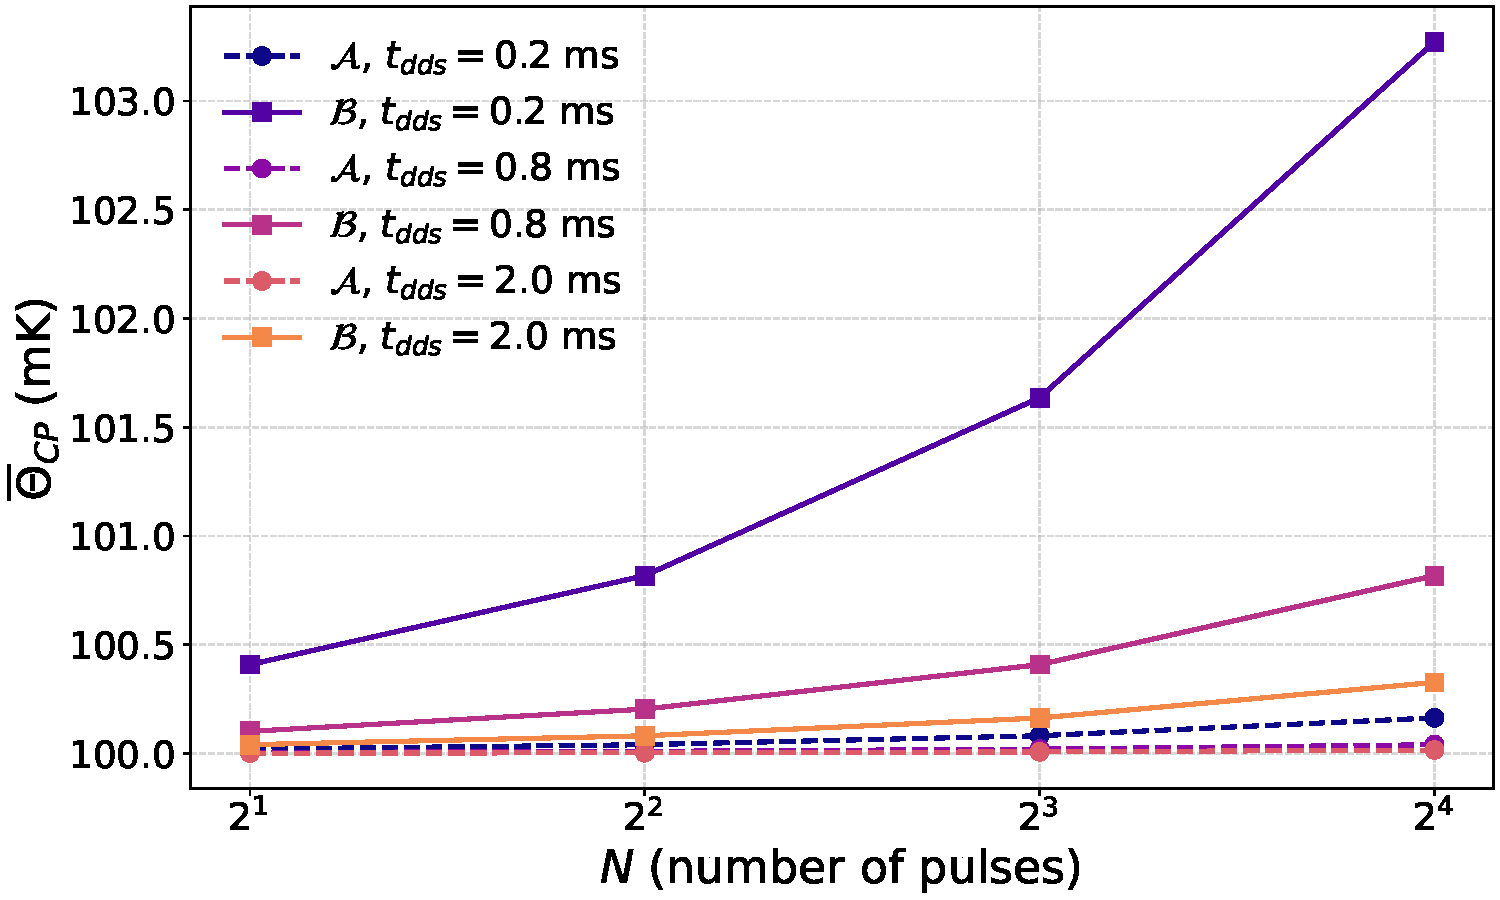
\includegraphics[width=0.7\linewidth]{figs/T_CP.pdf}
    \caption{Variation of average cold-plate stage temperature $\overline{\Theta}_{\text{CP}}$ with the number of pulses of CPMG sequence.}
    \label{fig:CPtemp}
\end{figure}

From, Eq. (80b), we get that the total heat load for unit pulse $\mathcal{A}$ driven at $\Omega_{\text{rabi,A}}=200$ M-rad/s, is $h_{A}\approx26.34~\mu$W. Since, pulse sequence $\mathcal{B}$ is an unoptimized pulse sequence, we get: $\Omega_{\text{rabi,B}}=\pi/t_{\pi,\text{B}}\approx 314.16$ M-rad/s. Since $P\propto\Omega^{2}$, we estimate that $h_{B}\approx65~\mu$W. After incorporating the duty cycle we get the following effective heat-loads for sequence $\mathcal{A}_{N}$ and $\mathcal{B}_{N}$ implementing a $N$-pulse CPMG:
\begin{subequations}
    \begin{align}
        \Tilde{h}_{\text{A}}(N) &= \text{dc}_{A}h_{A} \approx (0.79 N)~\text{nW}\\
        \Tilde{h}_{\text{B}}(N) &= \text{dc}_{B}h_{B} \approx (0.13 mN)~\text{nW}
    \end{align}
\end{subequations}
Given the effective heat-loads at the cold-plate, we use the calibration data from this reference \cite{krinner2019engineering}, to get an estimate of approximate rise in the temperature of the cold-plate stage. From this source \cite{krinner2019engineering}, we see that for heat load under 50 $\mu$W, the relative rise in cold-plate temperature is roughly linear, and is $\approx5.2\cdot10^{-3}/(\mu\text{W})$. Thus, the relative rise $\delta \overline{\Theta}/\overline{\Theta}_{\text{CP}}$ in average cold-plate temperature due to $\mathcal{A}_{N}$ and $\mathcal{B}_{N}$ is given by:
\begin{subequations}
    \begin{align}
        \frac{\delta \overline{\Theta}_{A}(N)} {\overline{\Theta}_{\text{CP}}} &\approx 4.11\cdot10^{-6} N\\
          \frac{\delta \overline{\Theta} _{B}(N)} {\overline{\Theta}_{\text{CP}}} &\approx 0.68\cdot10^{-6} m
        N
    \end{align}
\end{subequations}
Here, the overline corresponds to the ensemble average, over different cycles of the entanglement. Figure \ref{fig:CPtemp} plots the resulting average cold-plate temperature versus the number of pulses $N$ for multiple $t_{\text{dds}}$.

\subsubsection{Thermal Environment of Silicon Vacancy}
From the previous section, we estimated the heat-load in the sample is roughly $h_{\text{sample}}\approx\gamma_{\text{th}}0.084~\mu$W. We assume that the dynamic temperature of SiV$^{-}$ due to pulse incident at time $t_{0}$ is given by \cite{nguyen2019integrated}:
\begin{equation}
    \Theta_{\text{SiV}}(t,t_{0   }) = \Theta_{\text{CP}} + P_{\text{th}} (\text{e}^{-(t-t_{0})/\tau_{\text{th,SiV}}} - \text{e}^{-9(t-t_{0})/\tau_{\text{th,SiV}}})~\text{ReLU}(t-t_{0})
\end{equation}
Here, $P_{\text{th}}$ is a normalization constant, $\text{ReLU}$ is the rectified linear unit function. In the above expression, first term is the baseline temperature of the cold-plate, second term arises due to the slow thermalization of sample with the bath, and third term is due to the fast heating process due to the active heat-load on the sample. Suppose the volume of the diamond chip is $V_{\text{chip}}$. Since the Debye temperature of diamond is $\Theta_{\text{deb}}\approx 2230$ K \cite{mukherjee1967debye} 
and the operating temperature is within 1K, we can assume that the heat-capacity $C_{v}(\Theta)$ for diamond at temperature $\Theta$ is given by the Debye model:
\begin{align} 
    C_{v}(\Theta) &= \frac{12\pi^{4}}{5}\bigg(\frac{\Theta}{\Theta_{\text{deb}}}\bigg)^{3}N_{\text{atoms}}\text{k}_{\text{B}}
\end{align}
Here $N_{\text{atoms}}$ is the number of atoms of diamond in a chip of volume $V_{\text{chip}}$, and $\text{k}_{\text{B}}$ is the Boltzmann constant. For a typical chip footprint of $5\times5\times0.5$ mm$^{3}$, we get $C_{v}(\Theta=0.1\text{K})=6.42\cdot10^{-13}$ J/K. Suppose, the time $t_{0}$ at which pulse is applied the temperature of the SiV is $\Theta_{\text{SiV}}(t_{0})$, giving a heat-capacity of $C_{v}(\Theta_{\text{SiV}}(t_{0}))\equiv C_{v}(t_{0})$. We use the following approximation for estimating normalization constant $P_{\text{th}}$. We assume that the maximum temperature rise achieved by the sample is due to the total heat absorbed by the sample from the MW line, meaning: $h_{\text{sample}}t_{\pi}=C_{v}(\Theta^{\text{max}}_{\text{SiV}}-\Theta_{\text{CP}})$. After solving the above, we get the following: 
\begin{equation}
    P_{\text{th}}(t_{0}) \approx \frac{9~h_{\text{sample}}t_{\pi}}{8~\beta~C_{v}(t_{0})}
\end{equation}
$\beta = 9^{-1/8}$ arises by solving the derivative of Eq.(85). This gives the following expression for $\Theta_{\text{SiV}}$ for a single pulse:
\begin{equation}
    \Theta_{\text{SiV}}(t, t_{0}) = \Theta_{\text{CP}} + \frac{9~h_{\text{sample}}t_{\pi}}{8~\beta~C_{v}(t_{0})} (\text{e}^{-(t-t_{0})/\tau_{\text{th,SiV}}} - \text{e}^{-9(t-t_{0})/\tau_{\text{th,SiV}}})~\text{ReLU}(t-t_{0})
\end{equation}
Now, if instead of a single pulse, it is a pulse train incoming at integer multiples of $t_{0}$ i.e. \{$jt_{0}$\}, where $j$ is a natural number, then the temperature is given by:
\begin{equation}
    \Theta_{\text{SiV}}(t) = \Theta_{\text{CP}} + \sum_{j}\bigg(\Theta_{\text{SiV}}(t,jt_{0})-\Theta_{\text{CP}}\bigg)
\end{equation}

\begin{figure}
    \centering
    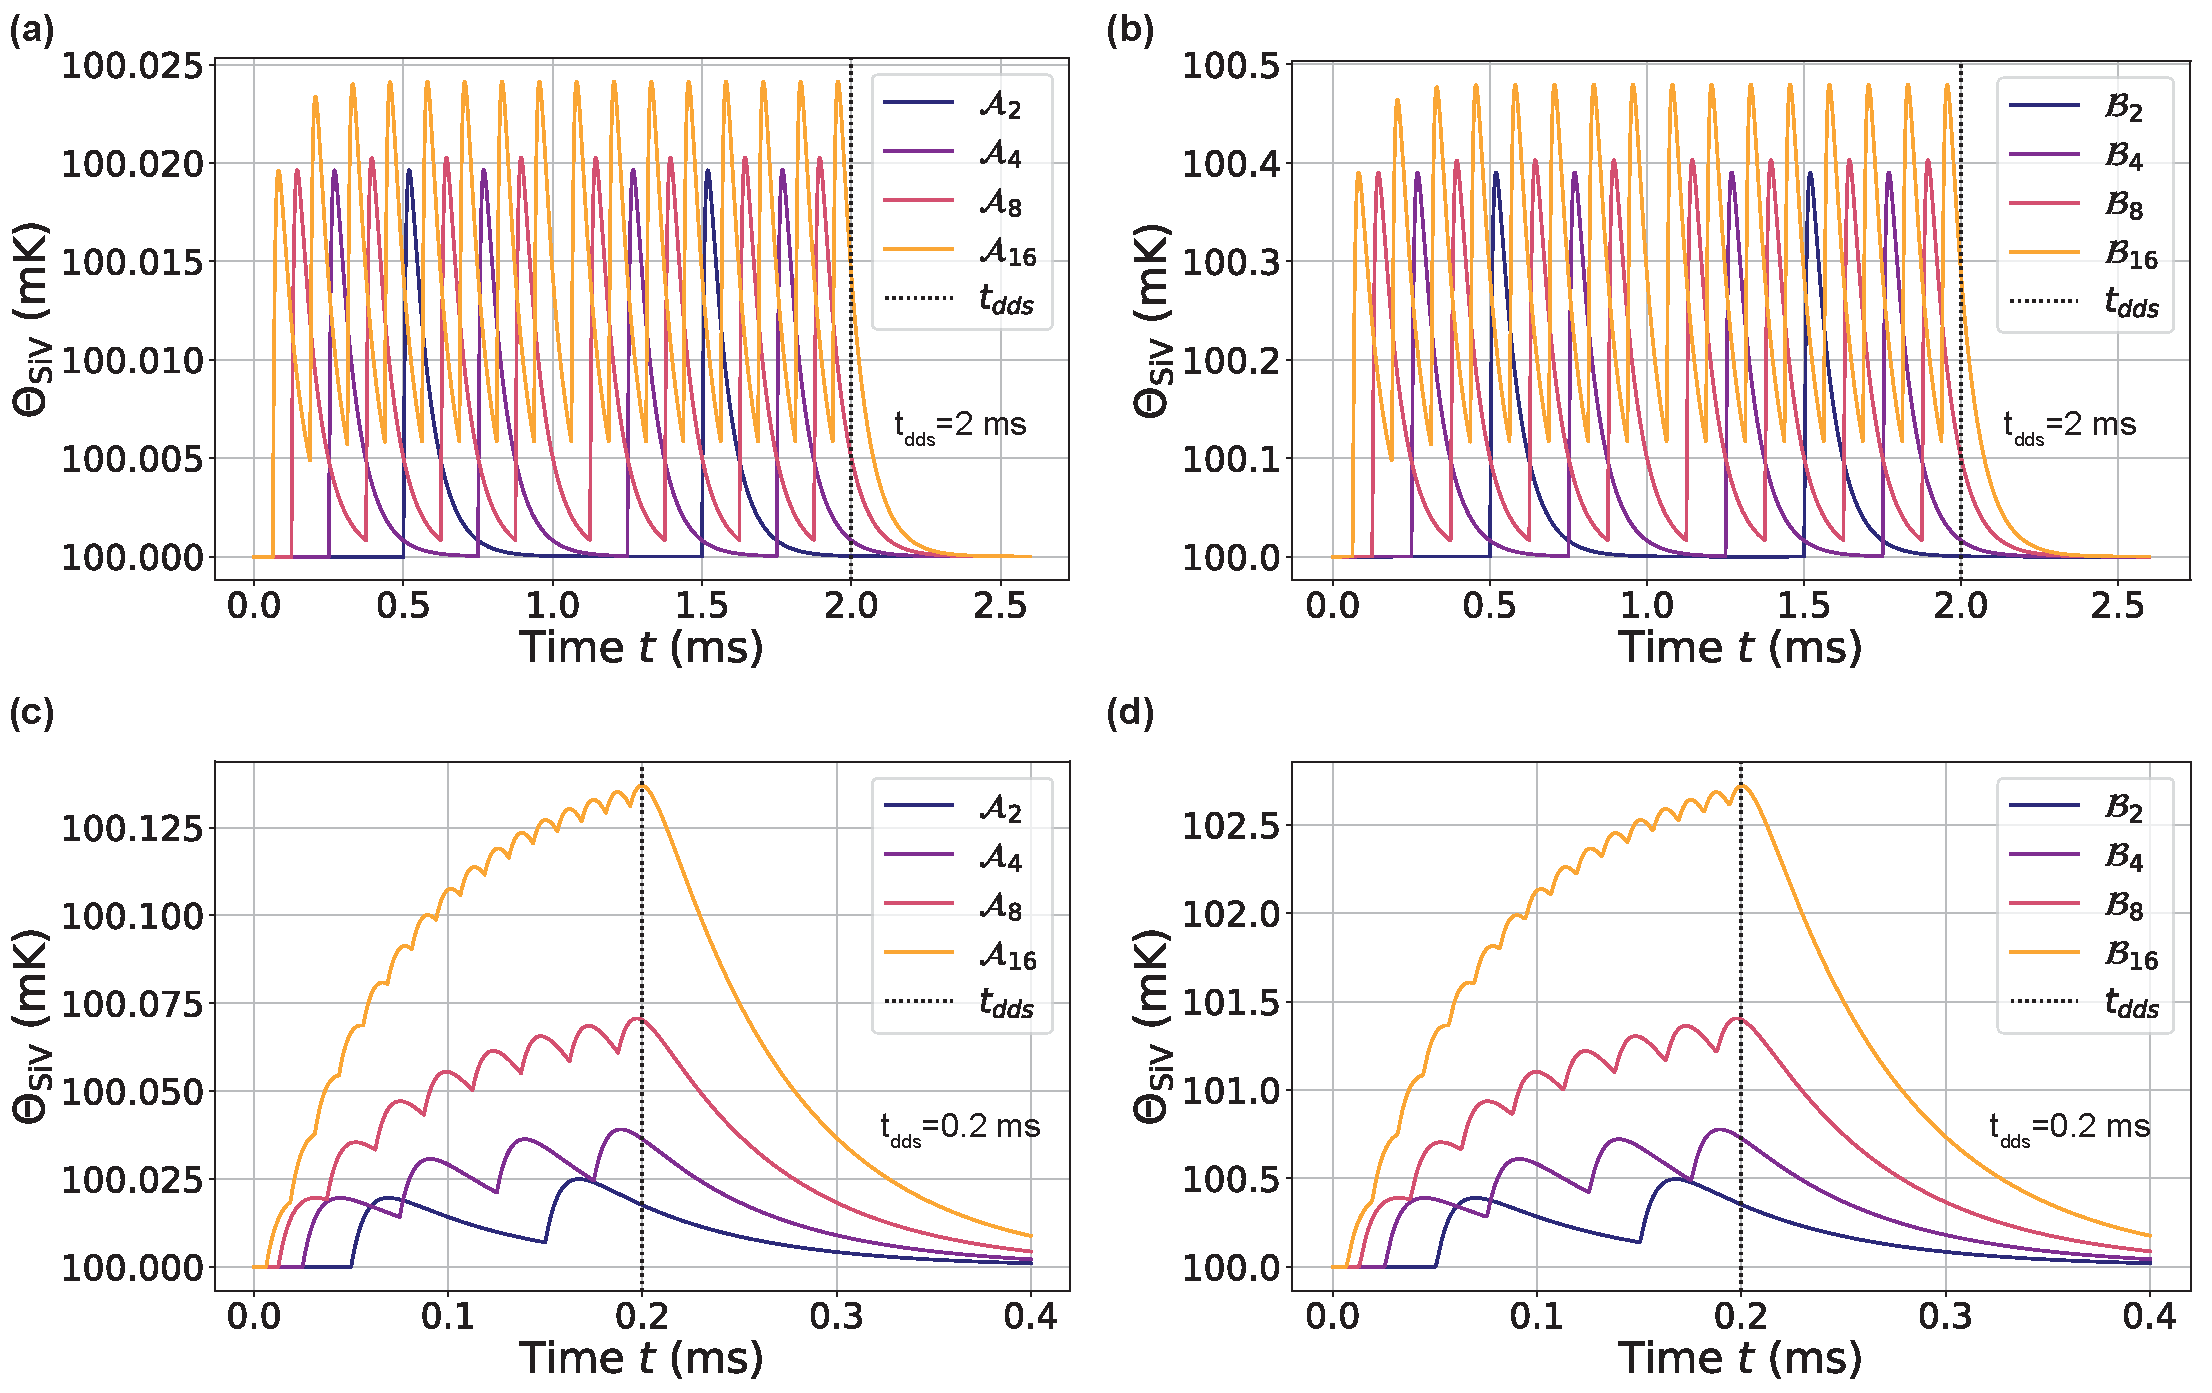
\includegraphics[width= \linewidth]{figs/T_SiV.pdf}
    \caption{\textbf{Variation of $\Theta_{\text{SiV}}$ with time.} Vertical dotted line shows the $t_{\text{dds}}$ mark where the dynamical decoupling sequence stops. \textbf{(a-b)} For large values of $t_{\text{dds}}=2$ ms, the incoming pulses are separated far enough for SiV to thermalize, that's why the temperature stays bounded. Sequence $\mathcal{B}$ leads to higher temperatures than $\mathcal{A}$ due to larger heat-load. \textbf{(c-d)} When the $t_{\text{dds}}$ is reduced to 0.2 ms, pulses are coming at a rate faster than the thermalization rate of SiV which leads to unbounded rise in average temperature with time until $t<t_{\text{dds}}$, after which the decoupling sequence ends and SiV starts to thermalize again. In this case also sequence $\mathcal{B}$ leads to higher temperatures than $\mathcal{A}$ due to larger heat-load.}
    \label{fig:sivtemperature}
\end{figure}

For sequence $\mathcal{A}_{N}$, pulse incoming times are $t_{j,A}=\{ \frac{(2j-1)t_{\text{dds}}}{2N} \}$, where $1\le j \le N$. For sequence $\mathcal{B}_{N}(m)$, the incoming times are $t_{jk,B}=\{ \frac{(2j-1)t_{\text{dds}}}{2N} + (k-1)t_{\pi,B}\}$, where $1\le j \le N$ and $1\le k \le m$. Thus, we get following SiV$^-$ temperatures for implementing both sequences:
\begin{subequations}
\begin{align}
    \Theta_{\text{SiV}}(t) &= \overline{\Theta}_{\text{CP}} + \sum^{N}_{j=1}\bigg(\Theta_{\text{SiV}}(t,t_{j,A})-\overline{\Theta}_{\text{CP}} \bigg)\hspace{35pt}: \text{For}~\mathcal{A}_{N}\\
    \Theta_{\text{SiV}}(t) &= \overline{\Theta}_{\text{CP}} + \sum^{N}_{j=1}\sum^{m}_{k=1}\bigg(\Theta_{\text{SiV}}(t,t_{jk,B}) - \overline{\Theta}_{\text{CP}}\bigg)\hspace{10pt}: \text{For}~\mathcal{B}_{N}(m)
\end{align}    
\end{subequations}


 Here, $\overline{\Theta}_{\text{CP}}$ takes into account the slow temperature rise in the cold-plate as in Eq.(84). In Fig. \ref{fig:sivtemperature}, we plot fast rise in $\Theta_{\text{SiV}}$ for $\mathcal{A}_{N}$ and $\mathcal{B}_{N}$, for different values of $N$, where we take $\overline{\Theta}_{\text{CP}}=100$ mK, in order to decouple the contribution from slow and fast rise in temperature. When the measurement window is large ($t_{\text{dds}}=2 $ ms), the SiV$^-$ gets time to re-thermalize between pulses, hence the temperature has a saw-tooth trend, and once the decoupling stops, the temperature thermalizes to $T_{\text{CP}}$. On the other hand, for low measurement time windows ($t_{\text{dds}}=0.2$ ms), there is less time for the SiV$^-$ to thermalize before the next pulse arrives, leading to the accumulation of heat and a rise in temperature with the incoming pulses. We measure the $T_{2}$, $T_{1}$ times of the silicon vacancy at the end of the measurement window (i.e. $t=t_{\text{dds}}$). We refer to this paper \cite{Sukachev_2017}, which measured $T^{*}_{2}\approx10~\mu$s  and $T_{1}\gtrsim1s$ (for $\Theta_{\text{SiV}} = 100$ mK). Further, we assume a linear dependence of $1/T^{*}_{2}$ ($\sim3~\text{MHz/K}$) and $1/T_{1}$ ($\sim2.4~\text{MHz/K}$) w.r.t. $\Theta_{\text{SiV}}$ \cite{Jahnke_2015}. If we assume that $z_{\text{dds}}\approx z_{\phi}\approx z_{\text{inh}}$, then we can further assume that $1/T_{2}$ also has a linear dependence on $\Theta_{\text{SiV}}$. Since, $T_{1}>>T^{*}_{2}$, we assume that $1/T_{2}$ has a similar scaling as $1/T^{*}_{2}$, which gives the following:
\begin{subequations}
    \begin{align}
       \frac{1}{T_{2}(\Theta_{\text{SiV}})} \left[1/\text{s}\right] &= \frac{1}{T_{2}(0.1~\text{K})} \left[1/\text{s}\right] + (\Theta_{\text{SiV}}-0.1)\cdot 3\cdot10^{6} \left[1/\text{K-s}\right]\\
       T_{2}(\Theta_{\text{SiV}}) &= \frac{T_{2}(0.1~\text{K})}{1 + T_{2}(0.1~\text{K})\cdot(\Theta_{\text{SiV}}-0.1)\cdot3\cdot10^{6}}
    \end{align}
\end{subequations}
Thus, we get the following effective $T_{2}$ times for a measurement window $t_{\text{dds}}$ for both sequences:
\begin{subequations}
    \begin{align}
       T_{2}(\Theta_{\text{SiV}}(t_{\text{dds}},\mathcal{A}_{N})) &= \frac{T_{2}(0.1~\text{K},\mathcal{A}_{N})}{1 + T_{2}(0.1~\text{K},\mathcal{A}_{N})\cdot(\Theta_{\text{SiV}}(t_{\text{dds}},\mathcal{A}_{N})-0.1)\cdot3\cdot10^{6}}\\[1.5ex]
       T_{2}(\Theta_{\text{SiV}}(t_{\text{dds}},\mathcal{B}_{N})) &= \frac{T_{2}(0.1~\text{K},\mathcal{B}_{N})}{1 + T_{2}(0.1~\text{K},\mathcal{B}_{N})\cdot(\Theta_{\text{SiV}}(t_{\text{dds}},\mathcal{B}_{N})-0.1)\cdot3\cdot10^{6}}
    \end{align}
\end{subequations}
Based on the slopes, we can write a similar expression for $T_{1}$:
\begin{subequations}
    \begin{align}
       T_{1}(\Theta_{\text{SiV}}(t_{\text{dds}},\mathcal{A}_{N})) &= \frac{T_{1}(0.1~\text{K},\mathcal{A}_{N})}{1 + T_{1}(0.1~\text{K},\mathcal{A}_{N})\cdot(\Theta_{\text{SiV}}(t_{\text{dds}},\mathcal{A}_{N})-0.1)\cdot2.4\cdot10^{6}}\\[1.5ex]
       T_{1}(\Theta_{\text{SiV}}(t_{\text{dds}},\mathcal{B}_{N})) &= \frac{T_{1}(0.1~\text{K},\mathcal{B}_{N})}{1 + T_{1}(0.1~\text{K},\mathcal{B}_{N})\cdot(\Theta_{\text{SiV}}(t_{\text{dds}},\mathcal{B}_{N})-0.1)\cdot2.4\cdot10^{6}}
    \end{align}
\end{subequations}
\newline
Since we now have a relation for the time-dependence of $T_{1}, T_{2}$, from Eq. (70), we can write the following:
\begin{equation}
    \epsilon_{jk}(\tau,N, T_{1}(\tau), T_{2j}(\tau), T_{2k}(\tau), z_{j,\text{dds}}, z_{k,\text{dds}} ) \equiv \epsilon_{jk}(\tau,N, z_{j,\text{dds}}, z_{k,\text{dds}})
\end{equation}
Since the entanglement process occurs in the time-window $t=(t_{\text{dds}}, t_{\text{dds}}+t_{\text{cmpl}})$, where $t_{\text{cmpl}}$ is the total time allocated for entanglement, we take the temporal average of Eq.(94), resulting in:

\begin{tcolorbox}[breakable, colback=white]
\begin{equation} 
    \overline{\epsilon_{jk}}(t_{\text{dds}}, t_{\text{cmpl}}, N, z_{j,\text{dds}}, z_{k,\text{dds}}) = \frac{1}{t_{\text{cmpl}}}\int^{t_{\text{dds}}+t_{\text{cmpl}}}_{t_{\text{dds}}}\epsilon_{jk}(\tau,N, z_{j,\text{dds}}, z_{k,\text{dds}})~\text{d}\tau
 \end{equation}
\end{tcolorbox}
We further change the number of qubits $m$ in sequence $\mathcal{B}(\tau,m)$ to see the impact on $\Theta_{\text{SiV}}$ and $T_{2}$ as seen in Fig.~\ref{fig:scaling}. As seen from the Fig.~\ref{fig:scaling}b, we observe that for larger value of $m$, the $T_{2}$ plot for $\mathcal{B}$ is completely submerged in the orange shaded region (signifying $T_{2}<t_{\text{dds}}$). This suggests that the pulse sequence stops to perform dynamical decoupling as we scale the number of qubits to be addressed.  

\begin{figure}
    \centering
    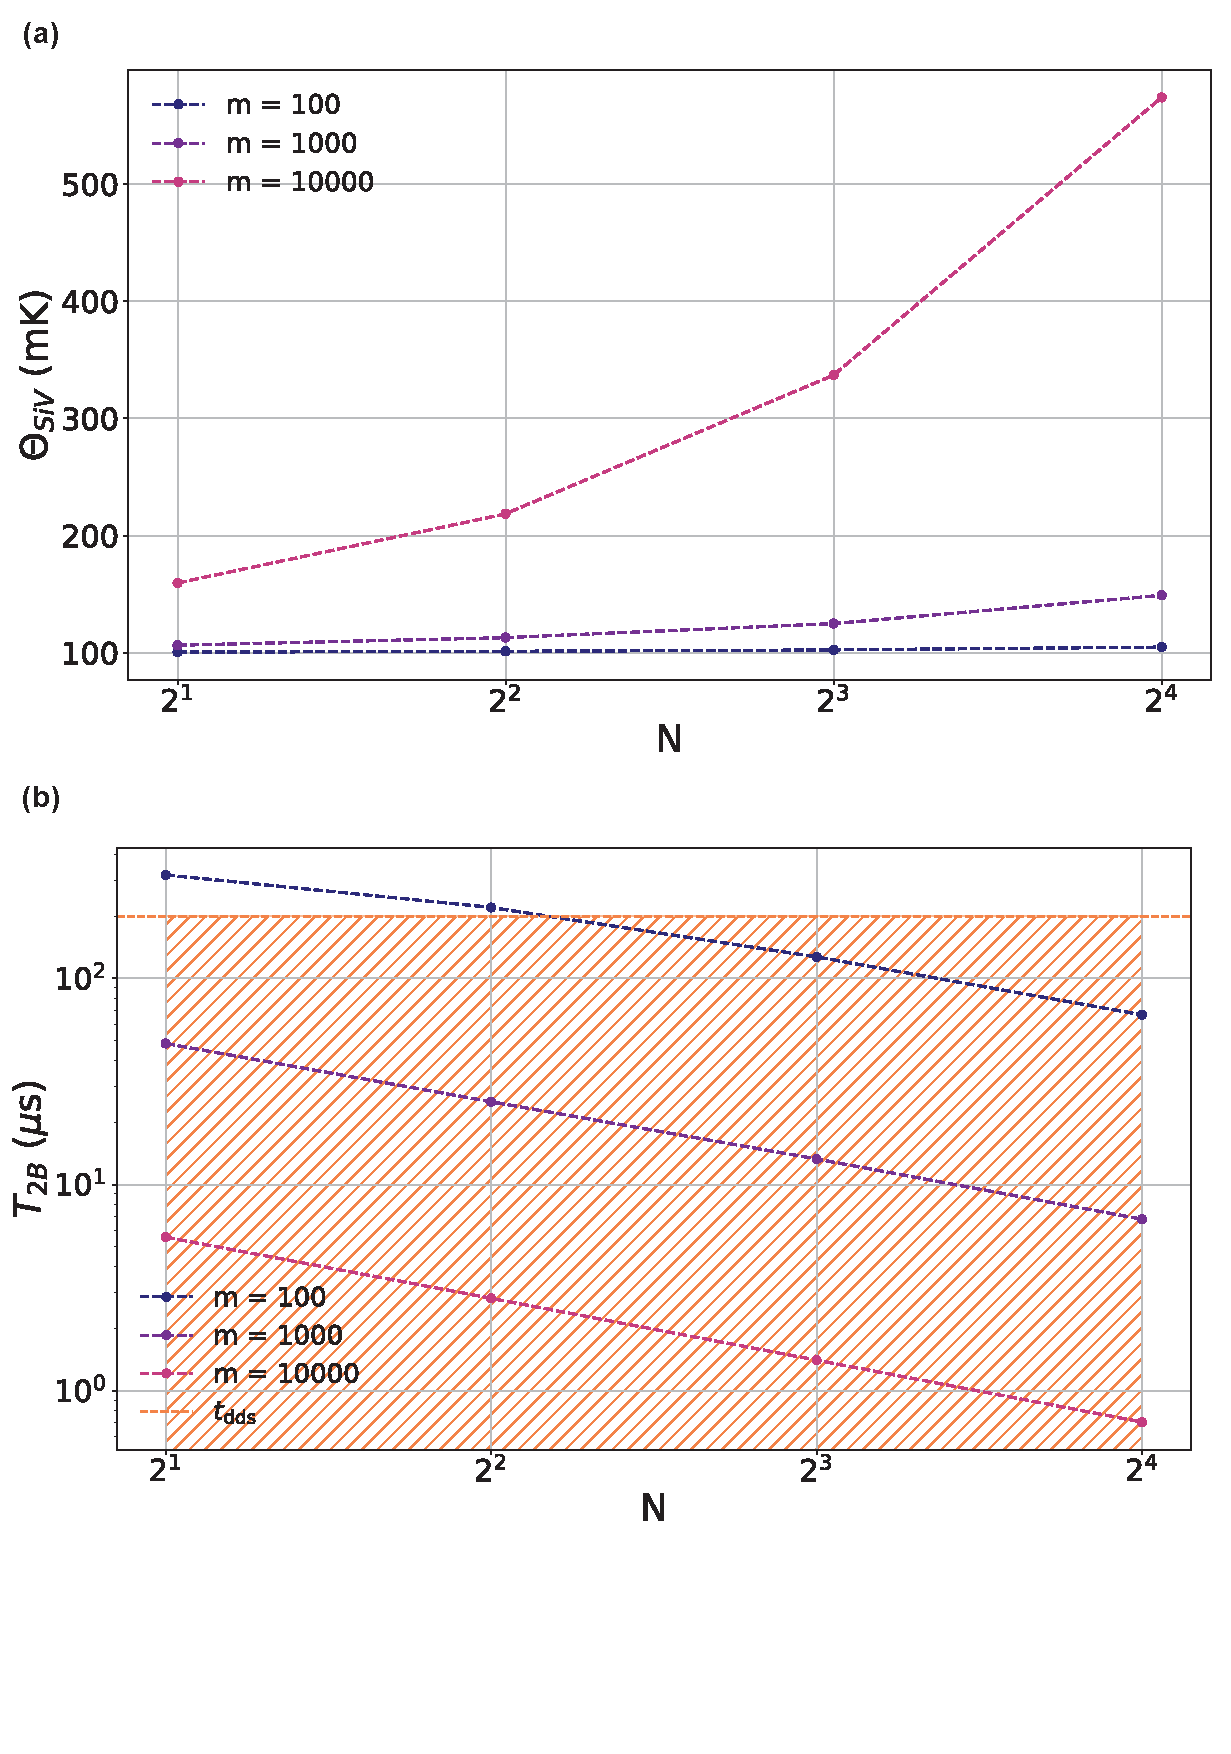
\includegraphics[width=0.8\linewidth]{figs/scaling.pdf}
    \caption{\textbf{Increasing the number of qubits}. \textbf{(a)} As the number of qubits $m$ increases from 100 to 10000, the heat-load due to pulse $\mathcal{B}$ increases, as seen from $\Theta_{\text{SiV}}$ due to $\mathcal{B}$ increasing by almost 4 times for $m=10000$ as $N$ changes from 2 to 16. \textbf{(b)} $T_{2}$ simulations for $\mathcal{B}$ for m = 1000 and 10000 are completely submerged in the orange shaded region which signifies the region $T_{2B} < t_{\text{dds}}$.
    }
    \label{fig:scaling}
\end{figure}


\newpage
\section{Derivation of the Fundamental Period $T$}

This derivation supports \textbf{Algorithm 2} from the main text by calculating the value of $\mathcal{J}$, which determines the minimum measurement window required to achieve the highest possible number of unique entanglement links. The calculation finds the fundamental period $T$ of the combined system, after which the pattern of entanglement attempts repeats. The value $\mathcal{J}$ is then determined from this period, setting the necessary number of attempts, $j_{\text{max}}$, to ensure all possible qubit pairs are brought into temporal coincidence at least once.\\

\textit{Setup.}

Device A has a sawtooth pattern of period $2T_a$:
\begin{align}
  \forall\,k\in\mathbb{Z}
  :\quad A(k + 2T_a) \;=\; A(k)
\end{align}

Device B has a sawtooth pattern of period $2T_b$ and runs at speed $d = \tfrac{p}{q}$, with $\gcd(p,q) = 1$:
\begin{gather}
\begin{cases}
    \forall\,k \in \mathbb{Z}:\; B(k + 2T_b) \;=\; B(k)\\
    \forall\,k\in\mathbb{Z}:\; B\!\bigl(\lfloor d\,k\rfloor \bigr) \;=\;
    B\!\Bigl(\left\lfloor \tfrac{p}{q}\,k \right\rfloor\Bigr) 
\end{cases}
\end{gather}

\textit{Definition of $T$.}

A positive integer $T$ is called a \emph{fundamental period} if
\begin{align}
   \forall\,k \in \mathbb{Z}
   :\quad
   A(k+T) = A(k)
   \;\;\;\wedge\;\;\;
   B\!\Bigl(\left\lfloor \tfrac{p}{q}(k+T)\right\rfloor\Bigr)
   \;=\;
   B\!\Bigl(\left\lfloor \tfrac{p}{q}\,k\right\rfloor\Bigr)
   \label{eq:fundamentalperiod}
\end{align}

We seek the minimal such $T$.

\textit{Condition for $A$.}

Since $A$ has period $2T_A$, we require
\begin{align}
   \forall\,k\in \mathbb{Z}
   :\quad
   A(k+T) = A(k)
   \quad\Longrightarrow\quad
   2T_a \;\mid\; T
\end{align}

\textit{Condition for $B$.}

We also require
\begin{align}
  \forall\,k \in \mathbb{Z}
  :\quad
  B\!\Bigl(\left\lfloor \tfrac{p}{q}(k+T)\right\rfloor\Bigr)
  \;=\;
  B\!\Bigl(\left\lfloor \tfrac{p}{q}\,k\right\rfloor\Bigr)
\end{align}

Since $B(\cdot)$ is $2T_b$--periodic in its integer input, it suffices that:

\begin{align}
    \forall\,k \in \mathbb{Z}: \quad
    \left\lfloor \tfrac{p}{q}(k+T)\right\rfloor 
    \;\equiv\;
    \left\lfloor \tfrac{p}{q}\,k\right\rfloor
    \pmod{2T_b}
\end{align}

A sufficient (and necessary) condition is:
\begin{align}
  \exists\,z \in \mathbb{Z}
  :\quad
  \frac{p}{q}\,T 
  \;=\;
  2T_b\,z.
\end{align}

\textit{Combining both conditions.}

$T$ must satisfy:
\begin{align}
   2T_a \;\mid\; T
   \quad\wedge\quad
   \exists\,z \in \mathbb{Z}
   :\;
   \frac{p\,T}{q} = 2T_b\,z
\end{align}

Equivalently, $2T_b\,q \,\mid\, p\,T$. Let $\gamma = \gcd\!\bigl(p,2T_b\,q\bigr)$, and write $p = \gamma\,p'$, $2T_b\,q = \gamma\,w$, with $\gcd(p',w)=1$. Then $2T_b\,q \mid p\,T$ is equivalent to $w \mid p'\,T$. Hence $T$ must be a multiple of $w$, and simultaneously a multiple of $2T_a$. The minimal positive $T$ satisfying both is:
\begin{align}
    T 
    \;=\;
    \mathrm{lcm}\!\Bigl(
      2T_a,
      \;\frac{2T_b\,q}{\gcd(p,\,2T_b\,q)}
    \Bigr).
\end{align}

This $T$ is the fundamental period, ensuring the condition of Eq. \ref{eq:fundamentalperiod}.

% \newpage
% \bibliography{bib}% Produces the bibliography via BibTeX.


% \newpage


\section{Quantum Sensing}

Color centers in diamond have been proven a promising platform for quantum sensing applications due to their remarkable sensitivity to external perturbations, such as magnetic and electric fields, temperature, and strain. Particularly, the negatively charged nitrogen vacancy (NV$^-$) center in diamond has been interesting for magnetometry due to its long spin coherence times at room temperature. One of the core concepts of this paper, resonantly applying a global control pulse simultaneously performing dynamical decoupling on an ensemble of color centers, can be easily extended from group-IV color centers to the NV$^-$ center. While the SAFE-GRAPE algorithm and dynamical decoupling sequence remain the same, the implementation of the control pulse is different. Instead of using strain driving, the control pulse can be implemented by microwave signals via an electromagnetic resonator.

By using an ensemble of $N_q$ color centers instead of a single one, the magnetometer's sensitivity can be enhanced by a factor $\sqrt{N_q}$. Current state-of-the-art ensemble-NV$^-$ magnetometers exhibit sensitivities down to the pT/$\sqrt{\text{Hz}}$ range. Consider the CPMG measurement sequence as our AC magnetometry protocol. The sensitivity $\eta$ in the presence of this dynamical decoupling is then given by \cite{RevModPhys.92.015004}: 

\begin{equation}
    \eta \approx \underbrace{\frac{\pi}{2}\frac{\hbar}{\Delta m_s g_e \mu_B} \frac{1}{\sqrt{N_q \tau}}}_{\text{spin projection limit}} \underbrace{\frac{1}{e^{-(\tau/T_2)^p}}}_{\text{spin decoherence}} \kappa_{\text{readout}} \kappa_{\text{duty}}
\end{equation}

Here $\Delta m_s=1$ as we use the effective $S=\frac{1}{2}$ NV$^-$ subspace, $g_e=2.003$ is the NV$^-$ electronic $g$ factor, $\mu_B$ is the Bohr magneton, $\tau$ is the interrogation time per measurement, $T_2$ is the coherence time and the stretched exponential parameter $p$ depends on the type of dephasing. There are two additional corrections: $\kappa_{\text{readout}}=\frac{1}{\mathcal{F}_{\text{readout}}}$ deals with the effect of imperfect readout fidelity $\mathcal{F}_{\text{readout}}$ and $\kappa_{\text{duty}}=\sqrt{\frac{t_I+\tau+t_R}{\tau}}$ takes into account the duty cycle, i.e. the fraction of interrogation time $\tau$ w.r.t. the total cycle time which also includes the initialization time $t_I$ and readout time $t_R$ of a measurement. 

Since $\eta \propto \frac{1}{\sqrt{N_q \tau}}$ for $\tau \lesssim T_2$, the sensitivity can be drastically improved by using the SAFE-GRAPE based composite pulse sequence for dynamical decoupling. This allows to achieve large $T_2$ for a large amount $N_q$ of color centers, which in turn lets you select a larger interrogation time $\tau$.

\endgroup
